\documentclass[journal,twocolumns]{IEEEtran}


% *** GRAPHICS RELATED PACKAGES ***
%
\ifCLASSINFOpdf
\usepackage[pdftex]{graphicx}
  % declare the path(s) where your graphic files are
  \graphicspath{{../Simulation/plots/}{../Proposal/}{../Kinematics/}}
  % and their extensions so you won't have to specify these with
  % every instance of \includegraphics
 % \DeclareGraphicsExtensions{.pdf,.jpeg,.png,.eps}
\else
  % or other class option (dvipsone, dvipdf, if not using dvips). graphicx
  % will default to the driver specified in the system graphics.cfg if no
  % driver is specified.
  % \usepackage[dvips]{graphicx}
  % declare the path(s) where your graphic files are
  % \graphicspath{{../eps/}}
  % and their extensions so you won't have to specify these with
  % every instance of \includegraphics
  % \DeclareGraphicsExtensions{.eps}
\fi
% graphicx was written by David Carlisle and Sebastian Rahtz. It is
% required if you want graphics, photos, etc. graphicx.sty is already
% installed on most LaTeX systems. The latest version and documentation
% can be obtained at: 
% http://www.ctan.org/tex-archive/macros/latex/required/graphics/
% Another good source of documentation is "Using Imported Graphics in
% LaTeX2e" by Keith Reckdahl which can be found at:
% http://www.ctan.org/tex-archive/info/epslatex/
%
% latex, and pdflatex in dvi mode, support graphics in encapsulated
% postscript (.eps) format. pdflatex in pdf mode supports graphics
% in .pdf, .jpeg, .png and .mps (metapost) formats. Users should ensure
% that all non-photo figures use a vector format (.eps, .pdf, .mps) and
% not a bitmapped formats (.jpeg, .png). IEEE frowns on bitmapped formats
% which can result in "jaggedy"/blurry rendering of lines and letters as
% well as large increases in file sizes.
%
% You can find documentation about the pdfTeX application at:
% http://www.tug.org/applications/pdftex


% Prof. Forbes math packages
\usepackage{amsmath} % cmex10
\usepackage{amssymb}
\usepackage{amsthm}
\usepackage{bm}
\usepackage{mathrsfs}
\usepackage{wrapfig}
\allowdisplaybreaks

%Units
\usepackage{siunitx}
\newcommand{\sii}[1]{\; [\si{#1}]}

%accents
\usepackage[latin1]{inputenc} 

\hyphenation{La-grange La-grang-ian dy-nam-ics}

% Matrix command
\newcommand{\bma}[1]{\left[\begin{array}{#1}}
\newcommand{\ema}{\end{array}\right]}
\newcommand{\trans}{{\ensuremath{\mathsf{T}}}} % transpose
\newcommand{\utimes}{ {\raisebox{-0.6ex}{ \kern-1.0ex\raisebox{0.6ex}{ \small $\mathsf{v}$}}} } % 
\newcommand{\onehalf}{\mbox{$\textstyle{\frac{1}{2}}$}}

% Bold symbols
\DeclareMathAlphabet{\mbf}{OT1}{ptm}{b}{n} % for bold face Roman
\newcommand{\mbs}[1]{{\boldsymbol{#1}}} % for bold face Greek

% Other bold symbols 
\newcommand{\mbfbar}[1]{{\bar{\mbf{#1}}}}
\newcommand{\mbfhat}[1]{{\hat{\mbf{#1}}}}
\newcommand{\mbftilde}[1]{{\tilde{\mbf{#1}}}}
\newcommand{\mbsbar}[1]{{\bar{\boldsymbol{#1}}}}
\newcommand{\mbshat}[1]{{\hat{\boldsymbol{#1}}}}
\newcommand{\mbstilde}[1]{{\tilde{\boldsymbol{#1}}}}

% Physical Space, physical vectors, a vectrix, etc. 
\newcommand{\pspace}{\mathbb{P}} 
\newcommand{\ura}[1]{{\underrightarrow{{#1}}}}
\newcommand{\vectrix}[1]{\ensuremath \underrightarrow{\boldsymbol{\mathcal{F}}}_{#1}}
\def\fdota{{\raisebox{-2pt}{\LARGE $\cdot$}}}
\def\fdotb{{\raisebox{-0.6ex}{ \kern0.2ex\raisebox{0.8ex}{\tiny $\hspace*{-1ex}\circ$}}}}
\def\fddota{{\raisebox{-2pt}{\LARGE $\cdot\hspace*{-0.2ex}\cdot$}}}
\def\fddotb{{\raisebox{-0.6ex}{ \kern0.2ex\raisebox{0.8ex}{\tiny $\hspace*{-1ex}\circ\circ$}}}}
\newcommand{\fdot}[1]{{^{\fdota{\mbox{\footnotesize${#1}$}}}}}
\newcommand{\fddot}[1]{{^{\fddota{\mbox{\footnotesize${#1}$}}}}}


% Short form for equations
\newcommand{\beq}{\begin{equation}}
\newcommand{\eeq}{\end{equation}}
\newcommand{\bdis}{\begin{displaymath}}
\newcommand{\edis}{\end{displaymath}}
\newcommand{\beqarray}{\begin{eqnarray}}
\newcommand{\eeqarray}{\end{eqnarray}}
\newcommand{\beqarraynn}{\begin{eqnarray*}}
\newcommand{\eeqarraynn}{\end{eqnarray*}}

%Must be equal to ...
\newcommand{\mbeq}{\overset{!}{=}}

% Matrices shortcut
\newcommand{\crossop}[3]{\bma{ccc} 0 & -#3 & #2 \\ #3 & 0 & -#1 \\ -#2 & #1 & 0 \ema}
\newcommand{\matr}[9]{\bma{ccc} #1 & #2 & #3 \\ #4 & #5 & #6 \\ #7 & #8 & #9 \ema}
\newcommand{\matrr}[4]{\bma{cc} #1 & #2  \\ #3 & #4  \ema}
\newcommand{\colvec}[3]{\bma{c} #1 \\ #2 \\ #3 \ema}
\newcommand{\rowvec}[3]{\bma{ccc} #1 & #2 & #3 \ema}
\newcommand{\colvecc}[2]{\bma{c} #1 \\ #2 \ema}
\newcommand{\rowvecc}[2]{\bma{cc} #1 & #2 \ema}
\newcommand{\Cone}[1]{\matr{1}{0}{0}{0}{\cos(#1)}{\sin(#1)}{0}{-\sin(#1)}{\cos(#1)}}
\newcommand{\Ctwo}[1]{\matr{\cos(#1)}{0}{-\sin(#1)}{0}{1}{0}{\sin(#1)}{0}{\cos(#1)}}
\newcommand{\Cthree}[1]{\matr{\cos(#1)}{\sin(#1)}{0}{-\sin(#1)}{\cos(#1)}{0}{0}{0}{1}}
\newcommand{\uo}{\ura{\omega}}
\newcommand{\ur}{\ura{r}}

\newcommand*\dif{\mathop{}\!\mathrm{d}}
\newcommand*\ex{\mathop{}\!\mathrm{ex}}
\newcommand{\sys}{\mathcal{A}}
\newcommand{\fbf}{\mbox{\textit{\textbf{f}}}}
\newcommand{\ddt}{\frac{\dif}{\dif t}}

\newcommand{\Sp}{\mathcal{S}}
\newcommand{\De}{\mathcal{D}}

\newcommand{\intd}{\int\displaylimits}

\begin{document}

\title{Final Report - ADR Spacecraft}
\IEEEpeerreviewmaketitle


\author{Fr�d�ric Berdoz, 260867318}% <-this % stops a space
\markboth{MECH 642 -- Advanced Dynamics}%
{Advanced Dynamics}

\maketitle
%%%%%%%%%%%%%%%%%%%%%%%%%%%%%%%%%%%%%%%%%%%%%%%%%%%%%%%%%%%%%%%%%%%%%%%%%
\section{Introduction} % Introduction of the system
\IEEEPARstart{S}{pace} debris are becoming a real threat to spacial exploration. Indeed, lower earth orbits (LEO) are slowly becoming saturated with loose objects and sending additional satellites or human missions is therefore becoming riskier. 

ESA, the European Space Agency, is now dedicating some of its ressources tracking these objects and planning their extraction or destruction. Their program is called \emph{Clean Space Initiative} \cite{eDeorbit}, and it involves ADR, standing for Active Debris Removal. It consists of sending spacecrafts in space that can either send the large and dangerous objects into higher orbits, known as graveyards, or slowing them down in order to initiate their reentry into the atmosphere, which would destroy them. In parallel, they are pressing governments to address this problem in their respective space law.

ESA's first planned ADR mission is called \emph{eDeorbit} and it has given rise to nummerous technical challenges, in particular in the field of robotics and advanced systems of guidance. They are currently exploring two options to catch the abandoned satellites.
\begin{enumerate}
\item A spacecraft with a robotic arm that can grip the object.
\item A spacecraft that can throw a net over the object.
\end{enumerate}
The objective of this project is to model a simplified version of the second design and to derive its equations of motion using the notation and the concepts exposed in \cite{Course}.
%%%%%%%%%%%%%%%%%%%%%%%%%%%%%%%%%%%%%%%%%%%%%%%%%%%%%%%%%%%%%%%%%%%%%%%%%
\section{Configuration of the Problem}
%General description of the system
The chosen design consists of a cylindrical spacecraft with one main propeller (P1), two auxiliary propellers (P2 \& P3), and two reaction wheels (W1 \& W2), as shown in Figure \ref{fig:Proposal}. 
Let $\mathcal{F}_e$ be the reference frame attached to the Earth, $o$ a point attached to the ground, $g_d$ the centre of masse of the debris and $\ura{v}^{g_do/e}$ the velocity of $g_d$ relative to $o$ w.r.t. $\mathcal{F}_e$. Let $A_d$ be the axis spanned by $\ura{v}^{g_do/e}$ and passing through $g_d$. The goal is to place the spacecraft's centre of mass on $A_d$, at a constant distance from $g_d$ and on the opposite direction of $\ura{v}^{g_do/e}$. Then, W1 and W2 can be used to align $A_s$ with $A_d$ such that the net launcher faces the debris. Once in position, the net launcher (NL) can be activated and the two auxiliary propellers can be used to slow down the debris just enough to initiate its reentry in the atmosphere.

In order to simplify the model, the following assumptions will be made:
\begin{itemize}
\item The curvature of the space is negligible compared to characteristic size of the problem, i.e. instead of considering a LEO, both objects are treated like they were in deep space. In this case, gravity is neglected.
\item The debris is free from external force, i.e. $\ura{v}^{g_do/e}$ is constant.
\item The total mass of the space craft and its inertia properties remain constant throughout the mission, i.e. the mass of the propellant used during the activation of P1, P2 and P3 is negligible.
\item The spacecraft fuselage, the two reaction wheels and the debris are modeled as continuous rigid bodies with constant density.
\end{itemize}
\begin{figure}[h!]
    \centering
        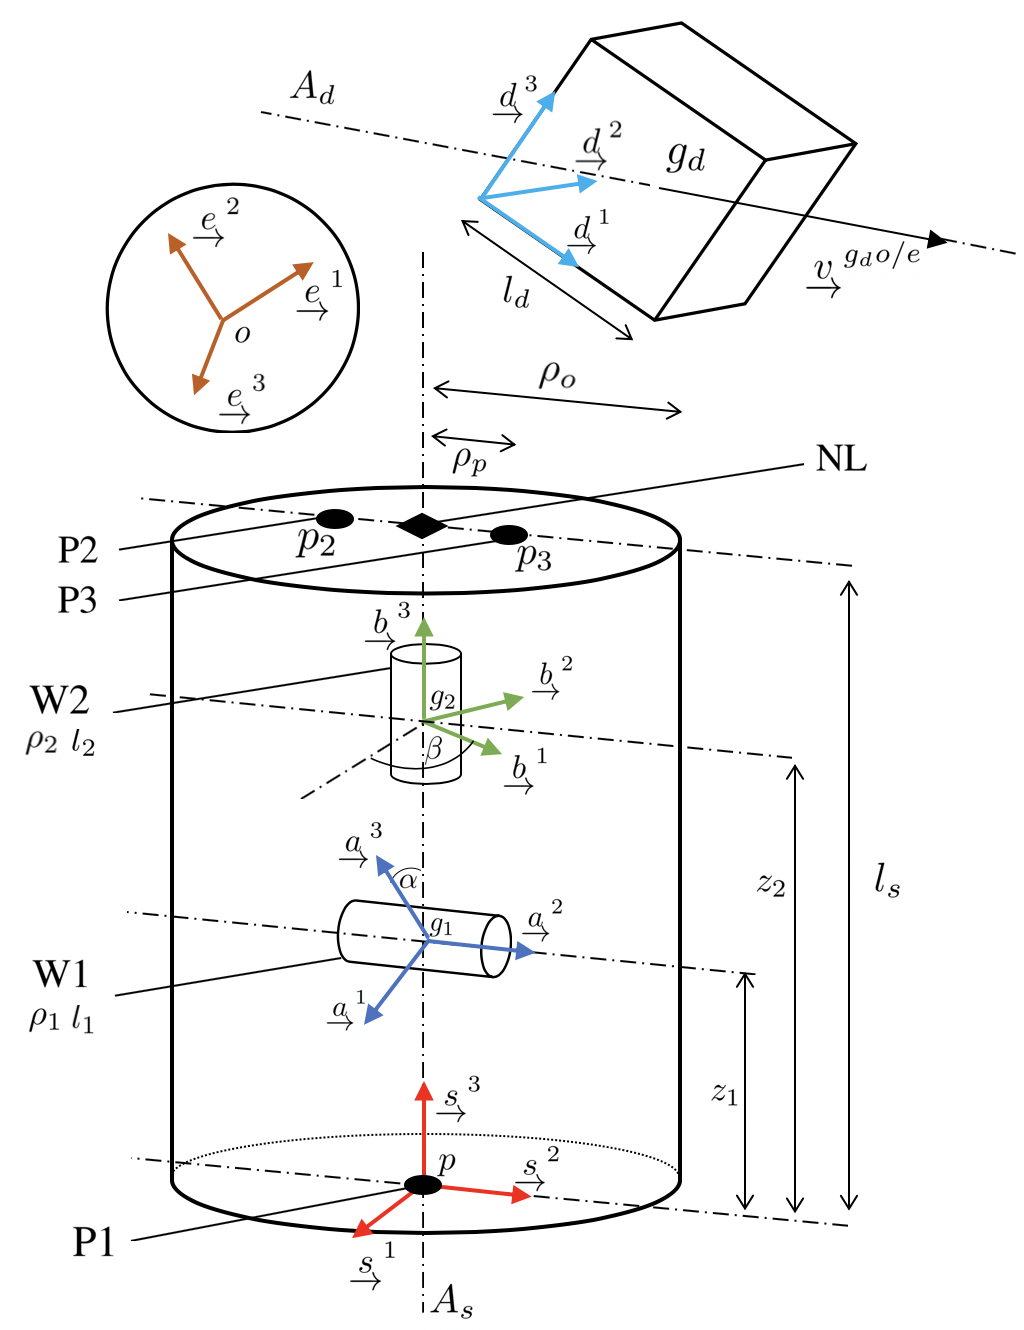
\includegraphics[width=.4\textwidth]{Final_Report_illustration}
    \caption{Spacecraft and debris configuration.}
    \label{fig:Proposal}
\end{figure}
%%%%%%%%%%%%%%%%%%%%%%%%%%%%%%%%%%%%%%%%%%%%%%%%%%%%%%%%%%%%%%%%%%%%%%%%%
\section{Geometrical Parameterization} \label{sec:Geometrical Parameterization}
%Introduction of the parameters
Let $\Sp$ and $\De$ denote the spacecraft fuselage and the debris, respectively, and let $\sys$ represent the whole system ($\Sp$+W1+W2+$\De$). The body $\Sp$ is modeled as a closed end hollow cylinder with a wall thickness $t_s$, an outer radius $\rho_o$ and a length $l_s$. Its main propeller P1 is attached to the main body at the point $p$, at the center of its base. On the top, the two auxiliary propellers P2 and P3 sit diametrically opposite each other, at a distance $\rho_p$ from $A_s$. The two reaction wheels W1 and W2 are modeled as full cylinders of radius and length $\rho_1$ and $l_1$ (respectively $\rho_2$ and $l_2$). W1 is oriented radially and W2 axially, in such a way that their centre of mass $g_{1}$ and $g_{2}$ are both on $A_s$. Moreover, W1 is aligned with P2 and P3. The length of point $g_{1}$ (and $g_{2}$) relative to point $p$ is $z_1$ (respectively $z_2$). The centre of mass of the wall $g_s$ coincide with the geometrical centre of the spacecraft. As for the debris, it is modeled as a full cube of size $l_d$. 
%%%%%%%%%%%%%%%%%%%%%%%%%%%%%%%%%%%%%%%%%%%%%%%%%%%%%%%%%%%%%%%%%%%%%%%%%
\section{Reference Frames}
For this problem, 5 different reference frames are considerd:
\begin{itemize}
\item $\mathcal{F}_e$ : An  inertial reference frame attached to the earth.
\item $\mathcal{F}_s$ : The reference frame attached to the body of the spacecraft. $\ura{s}^2$ is aligned with W1, $\ura{s}^3$ is aligned with $A_s$ and oriented towards the front of the spacecraft. Finally, $\ura{s}^1=\ura{s}^2\times\ura{s}^3$.
\item $\mathcal{F}_a$ : The reference frame attached to W1, obtained by rotating $\mathcal{F}_s$  about $\ura{s}^2=\ura{a}^2$. The angle of this rotation is refered to as $\alpha$.
\item $\mathcal{F}_b$ : The reference frame attached to W2, obtained by rotating $\mathcal{F}_s$  about $\ura{s}^3=\ura{b}^3$. The angle of this rotation is refered to as $\beta$.
\item $\mathcal{F}_d$ : The reference frame attached to the body of the debris and aligned with its edges.
\end{itemize}
%%%%%%%%%%%%%%%%%%%%%%%%%%%%%%%%%%%%%%%%%%%%%%%%%%%%%%%%%%%%%%%%%%%%%%%%%
\section{Attitude Description}
Since this problem is highly three dimensional, all the mutual configurations of the different reference frames are likely to happen. Using attitude parametrization that are not global or have kinematic singularities is risky and might in the end complicate the problem even more. This is why Direction Cosine Matrices will mostly be used. However, Euler Angles will be used to parameterize  $\mbf{C}_{as}$ and $\mbf{C}_{bs}$ in order to avoid excessive kinematic constraints. In fact, only one parameter is needed to describe each of them ($\alpha$ and $\beta$), and it will be shown later that this is a special case in which kinematic singularities are impossible. Moreover, this parameterization is global and its non uniqueness is not a problem since the exact values of $\alpha$ and $\beta$ are of poor value.
%%%%%%%%%%%%%%%%%%%%%%%%%%%%%%%%%%%%%%%%%%%%%%%%%%%%%%%%%%%%%%%%%%%%%%%%%
\section{Direction Cosine Matrices}
For this problem, the following 7 DCMs and their transpose will be used:
\begin{align}
\mbf{C}_{es} &=\mbf{C}_{se}^\trans=\rowvec{{\mbf{s}_e^1}}{{\mbf{s}_e^2}}{{\mbf{s}_e^3}}, \label{eq:Ces} \\
\mbf{C}_{ea} &=\mbf{C}_{ae}^\trans=\rowvec{{\mbf{a}_e^1}}{{\mbf{a}_e^2}}{{\mbf{a}_e^3}}, \label{eq:Cea} \\
\mbf{C}_{eb} &=\mbf{C}_{be}^\trans=\rowvec{{\mbf{b}_e^1}}{{\mbf{b}_e^2}}{{\mbf{b}_e^3}}, \label{eq:Ceb} \\
\mbf{C}_{ed} &=\mbf{C}_{de}^\trans=\rowvec{{\mbf{d}_e^1}}{{\mbf{d}_e^2}}{{\mbf{d}_e^3}}, \label{eq:Ced} \\
\mbf{C}_{sd}&=\mbf{C}_{ds}^\trans=\rowvec{{\mbf{d}_s^1}}{{\mbf{d}_s^2}}{{\mbf{d}_s^3}},  \label{eq:Csd} \\
\mbf{C}_{as}&=\mbf{C}_{sa}^\trans=\mbf{C}_2(\alpha),  \label{eq:Cas}\\
\mbf{C}_{bs}&=\mbf{C}_{sb}^\trans=\mbf{C}_3(\beta),  \label{eq:Cbs}
\end{align}
where $\mbf{C}_2(\alpha)$ and $\mbf{C}_3(\beta)$ are given by \eqref{eq:C2} and \eqref{eq:C3}.
%%%%%%%%%%%%%%%%%%%%%%%%%%%%%%%%%%%%%%%%%%%%%%%%%%%%%%%%%%%%%%%%%%%%%%%%%
\section{Angular Velocities}
Let $\mbf{q}^{xy}$ be the column matrix whose components are the columns of $\mbf{C}_{xy}^\trans$. In particular,
\bdis
\mbf{q}^{se}\triangleq\colvec{{\mbf{s}_e^1}}{{\mbf{s}_e^2}}{{\mbf{s}_e^3}}, \quad \mbf{q}^{ae}\triangleq\colvec{{\mbf{a}_e^1}}{{\mbf{a}_e^2}}{{\mbf{a}_e^3}}, \quad \mbf{q}^{be}\triangleq\colvec{{\mbf{b}_e^1}}{{\mbf{b}_e^2}}{{\mbf{b}_e^3}},
\edis
\bdis
\mbf{q}^{de}\triangleq\colvec{{\mbf{d}_e^1}}{{\mbf{d}_e^2}}{{\mbf{d}_e^3}}, \quad  \quad \mbf{q}^{ds}\triangleq\colvec{{\mbf{d}_s^1}}{{\mbf{d}_s^2}}{{\mbf{d}_s^3}}.
\edis
In this case, the angular velocities can be expressed in term of the parameters as follows:
\begin{align*}
\mbs{\omega}_s^{se}&=\mbf{S}_s^{se}\dot{\mbf{q}}^{se}, \\
\mbs{\omega}_a^{ae}&=\mbf{S}_a^{ae}\dot{\mbf{q}}^{ae},  \\
\mbs{\omega}_b^{be}&=\mbf{S}_b^{be}\dot{\mbf{q}}^{be},  \\
\mbs{\omega}_d^{de}&=\mbf{S}_d^{de}\dot{\mbf{q}}^{de},  \\
\mbs{\omega}_d^{ds}&=\mbf{S}_d^{ds}\dot{\mbf{q}}^{ds},  \\
\mbs{\omega}_a^{as}&=\mbf{S}_a^{as}\dot{\alpha},  \\
\mbs{\omega}_b^{bs}&=\mbf{S}_b^{bs}\dot{\beta}, 
\end{align*}
where the matrices $\mbf{S}_x^{xy}$ are derived in \cite{Slide8} and given by equations \eqref{eq:Ss_se} to \eqref{eq:Sb_bs}. Similarly, the inverse relations are 
\begin{align*}
\dot{\mbf{q}}^{se}&=\mbs{\Gamma}_s^{se}\mbs{\omega}_s^{se}, \\
\dot{\mbf{q}}^{ae}&=\mbs{\Gamma}_a^{ae}\mbs{\omega}_a^{ae}, \\
\dot{\mbf{q}}^{be}&=\mbs{\Gamma}_b^{be}\mbs{\omega}_b^{be}, \\
\dot{\mbf{q}}^{de}&=\mbs{\Gamma}_d^{de}\mbs{\omega}_d^{de}, \\
\dot{\mbf{q}}^{ds}&=\mbs{\Gamma}_d^{ds}\mbs{\omega}_d^{ds}, \\
\dot{\alpha}&=\mbs{\Gamma}_a^{as}\mbs{\omega}_a^{as}, \\
\dot{\beta}&=\mbs{\Gamma}_b^{bs}\mbs{\omega}_b^{bs}, \\
\end{align*}
where the matrices $\mbs{\Gamma}_x^{xy}$ are also derived in \cite{Slide8} and are given by equations \eqref{eq:Gs_se} to \eqref{eq:Gb_bs}. Lastly, let $\mbf{S}$ and $\mbs{\Gamma}$ be defined as follows:
\begin{align}
\mbf{S}&\triangleq \mbox{diag}\left\{\mbf{1},\mbf{S}_s^{se},\mbf{1},\mbf{S}_a^{ae},\mbf{1},\mbf{S}_b^{be},\mbf{1},\mbf{S}_d^{de}\right\}, \label{eq:S}\\
\mbs{\Gamma}&\triangleq \mbox{diag}\left\{\mbf{1},\mbs{\Gamma}_s^{se},\mbf{1},\mbs{\Gamma}_a^{ae},\mbf{1},\mbs{\Gamma}_b^{be},\mbf{1}, \mbs{\Gamma}_d^{d
e}\right\}. \label{eq:G}
\end{align}
%%%%%%%%%%%%%%%%%%%%%%%%%%%%%%%%%%%%%%%%%%%%%%%%%%%%%%%%%%%%%%%%%%%%%%%%%
\section{Components parameterization}
Due to the cylindrical symmetry of the spacecraft and the reaction wheels, the components of the physical vectors resolved in frame $\mathcal{F}_s$, $\mathcal{F}_a$ and $\mathcal{F}_b$ will be parametrized using the cylindrical coordinates. Let $\dif m_s$, $\dif m_1$ and $\dif m_2$ be material elements of the spacecraft wall, of W1 and of W2, respectively. The parametrization of the components of $\mbf{r}_s^{\dif m_sp}$, $\mbf{r}_a^{\dif m_1g_1}$ and $\mbf{r}_b^{\dif m_2g_2}$ will be done accordingly to Figure \ref{fig:Coordinates}.
\begin{figure}[h!]
    \centering
        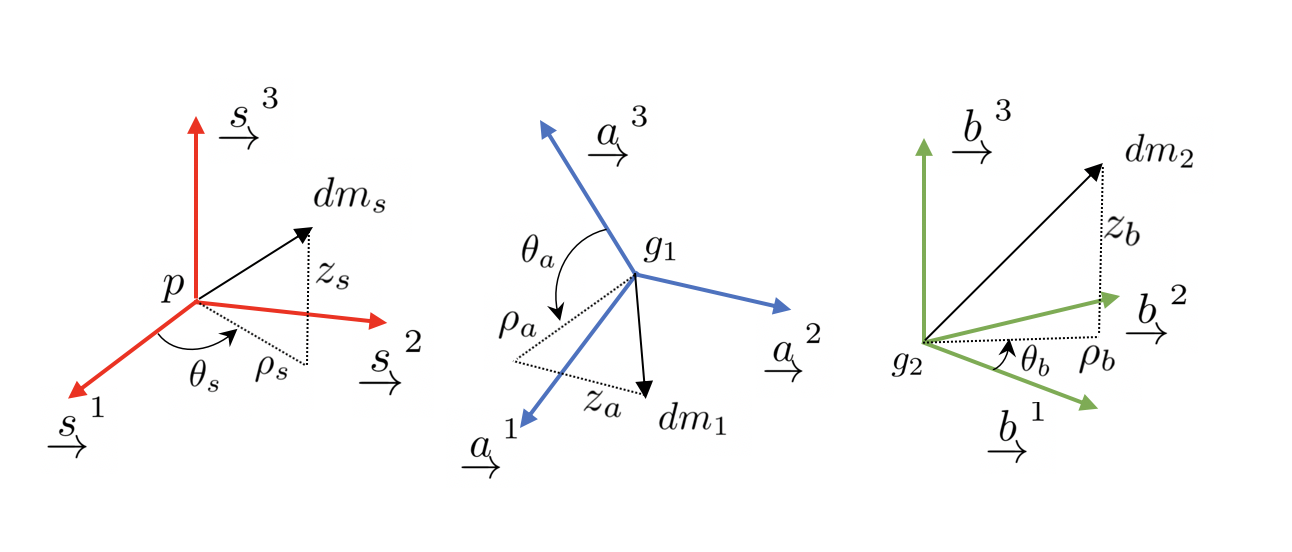
\includegraphics[width=.45\textwidth]{Kinematics_illustration2}
    \caption{Component parametrization in $\mathcal{F}_s$, $\mathcal{F}_a$ and $\mathcal{F}_b$.}
    \label{fig:Coordinates}
\end{figure}

As for the debris, the position of its material elements $\dif m_d$ relative to $g_d$ resolved in $\mathcal{F}_d$ will be described using a cartesian coordinate system. More precisely, $x_d$, $y_d$ and $z_d$ for the components along $\ura{d}^1$, $\ura{d}^2$ and $\ura{d}^3$, respectively.  In matrix form:
\begin{align*}
\mbf{r}_s^{dm_sp}=\colvec{\rho_s\cos(\theta_s)}{\rho_s\sin(\theta_s)}{z_s}, \quad & \mbf{r}_a^{dm_1g_1}=\colvec{\rho_a\cos(\theta_a)}{z_a}{\rho_a\sin(\theta_a)}, \\
\mbf{r}_b^{dm_2g_2}=\colvec{\rho_b\cos(\theta_b)}{\rho_b\sin(\theta_b)}{z_b}, \quad &  \mbf{r}_d^{dm_dg_d}=\colvec{x_d}{y_d}{z_d}.
\end{align*}
%%%%%%%%%%%%%%%%%%%%%%%%%%%%%%%%%%%%%%%%%%%%%%%%%%%%%%%%%%%%%%%%%%%%%%%%%
\section{State of the System}
% Introduction of the general coordinates, augmented velocities, reduced augmented velocities, augmented state and measurable state of the system.
This problem has 14 degrees of freedom (6 for the spacecraft, 1 for each reaction wheel and 6 for the debris). Therefore, in order to have a well defined and observable problem, at least 28 independent measurables are needed (14 positions and 14 velocities). The following assumptions will be made:
\begin{itemize}
\item The earth has a radar system that can determine $\mbf{r}_e^{g_do}$, $\mbf{v}^{g_do/e}_e$, $\mbf{r}_e^{po}$ and $\mbf{v}^{po/e}_e$. Moreover, it communicates with the spacecraft sensors in order to determine $\mbf{C}_{es}$. Lastly, it can compute $\mbs{\omega}_e^{se}$.
\item The spacecraft system knows $\alpha$, $\beta$, $\dot{\alpha}$ and $\dot{\beta}$.
\item The spacecraft has sensors that can observe the debris' behavior, i.e. $\mbf{C}_{sd}$ and $\mbs{\omega}_s^{ds}$  (It is assumed that the radars on earth are too far to observe directly the orientation and the spin of the debris).
\end{itemize}
It is useful to note that $\mbs{\omega}_e^{se}=\mbs{\omega}_s^{se}$ and $\mbs{\omega}_s^{ds}=\mbs{\omega}_d^{ds}$. In addition, let the column matrix $\bar{\mbf{x}}$ represent the measurable state of the system, whose components are simply the measurables.

On the other hand, in order to be able to treat the dynamic of each body separately, one can define the generalized coordinate $\mbf{q}$, the augmented velocities $\mbs{\nu}$ and the reduced augmented velocities $\hat{\mbs{\nu}}$ as follows:
\bdis
\mbf{q}
\triangleq\bma{c}
\mbf{r}_e^{po} \\
\mbf{q}^{se} \\
\mbf{r}_e^{g_1o} \\
\mbf{q}^{ae}  \\
\mbf{r}_e^{g_2o} \\
\mbf{q}^{be}  \\
\mbf{r}_e^{g_do} \\
\mbf{q}^{de}  \\
\ema,
\quad
\mbs{\nu}
%=\bma{c} \mbs{\nu}_s \\ \mbs{\nu}_a \\ \mbs{\nu}_b \\ \mbs{\nu}_d\ema
 \triangleq\bma{c}
\mbf{v}_e^{po/e} \\
\mbs{\omega}_s^{se} \\
\mbf{v}_e^{g_1o/e} \\
\mbs{\omega}_a^{ae}  \\
\mbf{v}_e^{g_2o/e} \\
\mbs{\omega}_b^{be}  \\
\mbf{v}_e^{g_do/e} \\
\mbs{\omega}_d^{de}  \\
\ema, 
\quad 
\hat{\mbs{\nu}}
 \triangleq\bma{c}
\mbf{v}_e^{po/e}  \\
\mbs{\omega}_s^{se} \\
\dot{\alpha} \\
\dot{\beta} \\
\mbf{v}_e^{g_do/e} \\
\mbs{\omega}_d^{de} 
\ema.
\edis
The relations between these three quantities are
\beq
\dot{\mbf{q}}=\mbs{\Gamma}\mbs{\nu}
\eeq
and
\beq
\mbs{\nu}=\mbs{\Pi}\hat{\mbs{\nu}}
\eeq
where $\mbs{\Gamma}$ and $\mbs{\Pi}$ are given by equations \eqref{eq:G} and \eqref{eq:Pi}, respectively. Lastly, one can define the augmented state of the system $\mbf{x}$ as follows:
\bdis
\mbf{x}\triangleq\colvecc{\mbf{q}}{\hat{\mbf{\nu}}}.
\edis
The relation between the measurable state and the augmented state is given by
\beq
\mbf{x}=\mbs{\Sigma}(\bar{\mbf{x}}),
\label{eq:xhatx}
\eeq
where $\mbs{\Sigma}(\bar{\mbf{x}})$ is defined by \eqref{eq:Sigma}. Here is a quick explanation why these different quantities are useful: $\mbf{q}$ and $\dot{\mbf{q}}$ are the generalized coordinates used in the Lagrange's Equation. However, expressing the kinetic energy directly in function of $\mbf{q}$ and  $\dot{\mbf{q}}$ can be tydious. This is why $\mbs{\nu}$ is introduced. Once the equations of motion are found in function of $\mbs{\nu}$, one can use $\hat{\mbs{\nu}}$ to perform the Null Space step so that the constraints disappear. Finally, one can use $\mbf{x}$ to transform the problem into a first order ODE that can be numerically integrated with the initial conditions $\mbf{x}_0=\mbs{\Sigma}(\bar{\mbf{x}}_0)$ where $\bar{\mbf{x}}_0$ are the measurables at time $t=0$. 
%%%%%%%%%%%%%%%%%%%%%%%%%%%%%%%%%%%%%%%%%%%%%%%%%%%%%%%%%%%%%%%%%%%%%%%%%
\section{Position}
One can now express the position, velocity and acceleration of each point relative to $o$ w.r.t. $\mathcal{F}_e$ and in functions of the measurables and their time derivative.
\begin{align}
\ura{r}^{dm_so} & = \vectrix{e}^\trans\left(\mbf{r}_e^{po}+\mbf{C}_{es}\mbf{r}_s^{dm_sp}\right), \\
\ura{r}^{dm_1o} & = \vectrix{e}^\trans\left(\mbf{r}_e^{po}+\mbf{C}_{es}\mbf{1}_3z_1+\mbf{C}_{es}\mbf{C}_{as}^\trans\mbf{r}_a^{dm_1g_1}\right), \\
\ura{r}^{dm_2o} & = \vectrix{e}^\trans\left(\mbf{r}_e^{po}+\mbf{C}_{es}\mbf{1}_3z_2+\mbf{C}_{es}\mbf{C}_{bs}^\trans\mbf{r}_b^{dm_2g_2}\right), \\
\ura{r}^{dm_do} & = \vectrix{e}^\trans\left(\mbf{r}_e^{g_do}+\mbf{C}_{es}\mbf{C}_{sd}\mbf{r}_d^{dm_dg_d}\right).
\end{align}
%%%%%%%%%%%%%%%%%%%%%%%%%%%%%%%%%%%%%%%%%%%%%%%%%%%%%%%%%%%%%%%%%%%%%%%%%
\section{Velocity}
\begin{align}
\ura{v}^{dm_so/e} & = \vectrix{e}^\trans\left(\mbf{v}_e^{po/e}+{\mbs{\omega}_{e}^{se}}^\times\mbf{C}_{es}\mbf{r}_s^{dm_sp}\right), 
\\ 
\ura{v}^{dm_1o/e} & = \vectrix{e}^\trans\left(\left[\mbf{C}_{es}\mbf{1}_2\dot{\alpha}+\mbs{\omega}_e^{se}\right]^\times\mbf{C}_{es}\mbf{C}_{as}^\trans\mbf{r}_a^{dm_1g_1}\right. 
\nonumber \\ & \quad \left. +\, {\mbs{\omega}_e^{se}}^\times\mbf{C}_{es}\mbf{1}_3z_1+\mbf{v}_e^{po/e} \right), 
\\ 
\ura{v}^{dm_2o/e} & = \vectrix{e}^\trans\left(\left[\mbf{C}_{es}\mbf{1}_3\dot{\beta}+\mbs{\omega}_e^{se}\right]^\times\mbf{C}_{es}\mbf{C}_{bs}^\trans\mbf{r}_b^{dm_2g_2}\right. 
\nonumber \\ & \quad \left. +\, {\mbs{\omega}_e^{se}}^\times\mbf{C}_{es}\mbf{1}_3z_2+\mbf{v}_e^{po/e} \right), 
\\ \ura{v}^{dm_do/e} & = \vectrix{e}^\trans\left( \left[\mbf{C}_{es}\mbs{\omega}_s^{ds}+\mbs{\omega}_e^{se}\right]^\times\mbf{C}_{es}\mbf{C}_{sd}\mbf{r}_d^{dm_dg_d}\right.
\nonumber\\ & \quad \left.+\mbf{v}_e^{g_do/e}\right).
\end{align}
%%%%%%%%%%%%%%%%%%%%%%%%%%%%%%%%%%%%%%%%%%%%%%%%%%%%%%%%%%%%%%%%%%%%%%%%%
\section{Acceleration}
\begin{align}
\ura{a}^{dm_so/e} & = \vectrix{e}^\trans\left(
\dot{\mbf{v}}_e^{po/e}+\left.\dot{\mbs{\omega}}_e^{se}\right.^\times\mbf{C}_{es}\mbf{r}_s^{dm_sp}
\right. \nonumber \\ & \quad \left.
+\,{\mbs{\omega}_e^{se}}^\times{\mbs{\omega}_e^{se}}^\times\,\mbf{C}_{es}\mbf{r}_s^{dm_sp}
\right), 
\\
\ura{a}^{dm_1o/e} & = \vectrix{e}^\trans\left(
\left[\mbf{C}_{es}\mbf{1}_2\ddot{\alpha}+\dot{\mbs{\omega}}_e^{se}
-\mbf{C}_{es}(\mbf{1}_2\dot{\alpha})^\times\mbs{\omega}_e^{se}\right]^\times \dots
\right. \nonumber \\ & \quad \left.
\mbf{C}_{es}\mbf{C}_{as}^\trans\mbf{r}_a^{dm_1g_1}
+\left[\mbf{C}_{es}\mbf{1}_2\dot{\alpha}+\mbs{\omega}_e^{se}\right]^\times \dots
\right. \nonumber \\ & \quad \left.
\left[\mbf{C}_{es}\mbf{1}_2\dot{\alpha}+\mbs{\omega}_e^{se}\right]^\times\mbf{C}_{es}\mbf{C}_{as}^\trans\mbf{r}_a^{dm_1g_1}
\right. \nonumber \\ & \quad \left.
+\left[\left.\dot{\mbs{\omega}}_e^{se}\right.^\times+{\mbs{\omega}_e^{se}}^\times{\mbs{\omega}_e^{se}}^\times\right]\mbf{C}_{es}\mbf{1}_3z_1
\right. \nonumber \\ & \quad \left.
+\,\dot{\mbf{v}}_e^{po/e}
\right), 
\\
\ura{a}^{dm_2o/e} & = \vectrix{e}^\trans\left(
\left[\mbf{C}_{es}\mbf{1}_3\ddot{\beta}+\dot{\mbs{\omega}}_e^{se}
-\mbf{C}_{es}(\mbf{1}_3\dot{\beta})^\times\mbs{\omega}_e^{se}\right]^\times \dots
\right. \nonumber \\ & \quad \left.
\mbf{C}_{es}\mbf{C}_{bs}^\trans\mbf{r}_b^{dm_2g_2}
+\left[\mbf{C}_{es}\mbf{1}_3\dot{\beta}+\mbs{\omega}_e^{se}\right]^\times \dots
\right. \nonumber \\ & \quad \left.
\left[\mbf{C}_{es}\mbf{1}_3\dot{\beta}+\mbs{\omega}_e^{se}\right]^\times\mbf{C}_{es}\mbf{C}_{bs}^\trans\mbf{r}_b^{dm_2g_2}
\right. \nonumber \\ & \quad \left.
+\left[\left.\dot{\mbs{\omega}}_e^{se}\right.^\times+{\mbs{\omega}_e^{se}}^\times{\mbs{\omega}_e^{se}}^\times\right]\mbf{C}_{es}\mbf{1}_3z_2
\right. \nonumber \\ & \quad \left.
+\,\dot{\mbf{v}}_e^{po/e}
\right), 
\\
\ura{a}^{dm_do/e} & = \vectrix{e}^\trans\left(
\left[\mbf{C}_{es}\dot{\mbs{\omega}}_s^{ds}+\dot{\mbs{\omega}}_e^{se}-\left\{\mbf{C}_{es}\mbs{\omega}_s^{ds}\right\}^\times\mbs{\omega}_e^{se}\right]^\times \dots
\right. \nonumber \\ & \quad \left.
\mbf{C}_{es}\mbf{C}_{sd}\mbf{r}_d^{dm_dg_d}
\right. \nonumber \\ & \quad \left.
+\left[\mbf{C}_{es}\mbs{\omega}_s^{ds}+\mbs{\omega}_e^{se}\right]^\times\left[\mbf{C}_{es}\mbs{\omega}_s^{ds}+\mbs{\omega}_e^{se}\right]^\times \dots
\right. \nonumber \\ & \quad \left.
\mbf{C}_{es}\mbf{C}_{sd}\mbf{r}_d^{dm_dg_d}+\dot{\mbf{v}}_e^{g_do/e}
\right).
\end{align}
%%%%%%%%%%%%%%%%%%%%%%%%%%%%%%%%%%%%%%%%%%%%%%%%%%%%%%%%%%%%%%%%%%%%%%%%%
\section{Approach}
%Description of the approach taken in order to derive the equtions of motion.
In order to derive the equations of motion, the Lagrangian approach will be used. It has the advantage of not involving any internal force. Moreover, it allows to treat each body of the system separately. Their motions are then coupled together by simply introducing attitude and collocation constraints, which is precisely what is done in the end part of this report.
%%%%%%%%%%%%%%%%%%%%%%%%%%%%%%%%%%%%%%%%%%%%%%%%%%%%%%%%%%%%%%%%%%%%%%%%%
\section{Mass Properties}
In order to shorten the notation, let $\mbs{\digamma}^{\mathcal{B}}(\mbf{x})$ denote the integration of the quantity $\mbf{x}$ (scalar or matrix) over the body $\mathcal{B}$. In particular, using the the parameters defined in section \ref{sec:Geometrical Parameterization}, $\mbs{\digamma}^{\Sp}(\mbf{x})$, $\mbs{\digamma}^{W1}(\mbf{x})$, $\mbs{\digamma}^{W2}(\mbf{x})$ and $\mbs{\digamma}^{\De}(\mbf{x})$ are given by equations \eqref{eq:FS} to \eqref{eq:FD}.
Let $V_s$, $V_1$, $V_2$ and $V_d$ be the volume of $\Sp$, W1, W2 and $\De$, respectively. They are simply given by:
\begin{align*}
V_s=\mbs{\digamma}^{\Sp}(1),
& \quad
V_1=\mbs{\digamma}^{W1}(1),
& 
V_2=\mbs{\digamma}^{W2}(1), 
& \quad
V_d=\mbs{\digamma}^{\De}(1).
\end{align*}
Therefore, since the densities are assumed to be constant, the corresponding masses become:
\begin{align*}
m_s=\sigma_sV_s,
& \quad
m_1=\sigma_1V_1,
& 
m_2=\sigma_2V_2, 
& \quad
m_d=\sigma_dV_d.
\end{align*}
%Lastly,
%\bdis
%m_\mathcal{A}=m_s+m_1+m_2.
%\edis
The relevant first moments of mass of each body are given by:
\begin{align*}
&\ura{c}^{\Sp p}=m_s\ur^{g_s p}=\rowvec{0}{0}{\onehalf m_s l_s}\vectrix{s},
\\
%&\ura{c}^{W1 p}= \rowvec{0}{0}{m_1z_1}\vectrix{s},
%\\
%&\ura{c}^{W2 p}= \rowvec{0}{0}{m_2z_2}\vectrix{s},
%\\
&\ura{c}^{W1 g_1}=\ura{c}^{W2 g_2}=\ura{c}^{\De g_d}=\ura{0}.
\end{align*}
Similarly, using the following identities:
\bdis
\ura{J}^{\mathcal{B}z}=\vectrix{b}^\trans\mbf{J}_b^{\mathcal{B}z}\vectrix{b}, \quad \mbf{J}_b^{\mathcal{B}z}=-\int_{\mathcal{B}}{\mbf{r}_b^{\dif mz}}^\times{\mbf{r}_b^{\dif mz}}^\times \dif m,
\edis
one can compute the second moments of mass of each body resolved in their respective body frame. In particular,
\begin{align*}
&\mbf{J}_s^{\Sp p}=\mbs{\digamma}^{\Sp}(-\sigma_s{\mbf{r}_s^{\dif m_sp^\times}}{\mbf{r}_s^{\dif m_sp^\times}}),
\\
&\mbf{J}_a^{W1 g_1}=\mbs{\digamma}^{W1}(-\sigma_1{\mbf{r}_a^{\dif m_1g_1^\times}}{\mbf{r}_a^{\dif m_1g_1^\times}}),
\\
&\mbf{J}_b^{W2 g_2}=\mbs{\digamma}^{W2}(-\sigma_2{\mbf{r}_b^{\dif m_2g_2^\times}}{\mbf{r}_b^{\dif m_2g_2^\times}}),
\\
&\mbf{J}_d^{\De g_d}=\mbs{\digamma}^{\De}(-\sigma_d{\mbf{r}_d^{\dif m_dg_d^\times}}{\mbf{r}_d^{\dif m_dg_d^\times}}),
%\\
%&\mbf{J}_s^{W1 p}=-m_1{\mbf{r}_s^{g_1p^\times}}{\mbf{r}_s^{g_1p^\times}},
%\\
%&\mbf{J}_s^{W2 p}=-m_2{\mbf{r}_s^{g_2p^\times}}{\mbf{r}_s^{g_2p^\times}},
%\\ &
%\mbf{J}_s^{\mathcal{A}p}=\mbf{J}_s^{\Sp p}+\mbf{J}_s^{W1 p}+\mbf{J}_s^{W2 p}.
\end{align*}
where the argument of each body integration is given  explicitly  by \eqref{eq:rSx},  \eqref{eq:rW1x}, \eqref{eq:rW2x} and \eqref{eq:rDx}, respectivley.
This allows to define the following mass matrices:
%\footnotesize
\begin{align*}
\mbf{M}^{\Sp p}&\triangleq\matrr{m_s\mbf{1}}{-\mbf{C}_{es}{\mbf{c}_s^{\Sp p}}^\times}{{\mbf{c}_s^{\Sp p}}^\times\mbf{C}_{es}^\trans}{\mbf{J}_s^{\Sp p}}, 
\\
\mbf{M}^{W1 g_1}&\triangleq\matrr{m_1\mbf{1}}{\mbf{0}}{\mbf{0}}{\mbf{J}_a^{W1 g_1}},
 \\
\mbf{M}^{W2 g_2}&\triangleq\matrr{m_2\mbf{1}}{\mbf{0}}{\mbf{0}}{\mbf{J}_b^{W2 g_2}}, 
\\
\mbf{M}^{\De g_d}&\triangleq\matrr{m_d\mbf{1}}{\mbf{0}}{\mbf{0}}{\mbf{J}_d^{\De g_d}}, 
\end{align*}
Finally, one can define the mass matrix of the whole system as
\beq
\mbf{M}\triangleq\mbox{diag}\left\{\mbf{M}^{\Sp p},\mbf{M}^{W1 g_1},\mbf{M}^{W2 g_2},\mbf{M}^{\De g_d}\right\}.
\label{eq.M}
\eeq
\normalsize
%%%%%%%%%%%%%%%%%%%%%%%%%%%%%%%%%%%%%%%%%%%%%%%%%%%%%%%%%%%%%%%%%%%%%%%%%
\section{Control}
The spacecraft has three linear actuators (P1, P2 and P3) and two rotary actuators (W1 and W2). The direction of the thrust produced by the propellers is assumed to remain perpendicular to the surface of the spacecraft, and directed towards it (no pull). Let $p$, $p_2$ and $p_3$ be the points where the actuators P1, P2 and P3 are fixed to the spacecraft, respectively. Under these assumptions,
\begin{align*}
\ura{f}^{p}&=\rowvec{0}{0}{f^{P1}}\vectrix{s},
\\ 
\ura{f}^{p_2}&=\rowvec{0}{0}{-f^{P2}}\vectrix{s},
\\
\ura{f}^{p_3}&=\rowvec{0}{0}{-f^{P3}}\vectrix{s}.
\end{align*}
Additionally, let $\ura{\tau}^{W1 \Sp}$ and $\ura{\tau}^{W2 \Sp}$ be the torques applied on W1 and W2 by the actuators placed on the spacecraft wall. From Newton's third law, the torques applied on the wall by the reaction wheels, $\ura{\tau}^{\Sp W1}$ and $\ura{\tau}^{ \Sp W2}$, are simply given by
\bdis
\ura{\tau}^{\Sp W1}=-\ura{\tau}^{W1\Sp}, \quad \ura{\tau}^{\Sp W2}=-\ura{\tau}^{W2\Sp}.
\edis
Resolving these physical vectors in the body frames yields
\begin{align*}
\ura{\tau}^{W1 \Sp}&=\rowvec{0}{\tau^{W1}}{0}\vectrix{a},\\
\ura{\tau}^{\Sp W1}&=\rowvec{0}{-\tau^{W1}}{0}\vectrix{s}, \\
\ura{\tau}^{W2\Sp}&=\rowvec{0}{0}{\tau^{W2}}\vectrix{b}, \\
 \ura{\tau}^{\Sp W2}&=\rowvec{0}{0}{-\tau^{W2}}\vectrix{s}.
\end{align*}
Therefore, the behavior of the system only depends on the initial configuration and the following controllable (time-dependent) quantity: 
\bdis
\mathfrak{f}\triangleq\bma{ccccc} f^{P1} & f^{P2} & f^{P3} & \tau^{W1} & \tau^{W2} \ema^\trans.
\edis
In this case, the generalized forces and moments with respect to $\mbf{q}$ are given by
\beq
\mbs{f}=\mbf{B}\mathfrak{f}, \quad 
\mbf{B}\triangleq\bma{c}
\mbf{B}_s \\
\mbf{B}_a \\
\mbf{B}_ b \\
 \mbf{0}
\ema,
\eeq
where $\mbf{B}_s$, $\mbf{B}_a$ and $\mbf{B}_b$ are given by \eqref{eq:Bs}, \eqref{eq:Ba} and \eqref{eq:Bb}, respectively.
%%%%%%%%%%%%%%%%%%%%%%%%%%%%%%%%%%%%%%%%%%%%%%%%%%%%%%%%%%%%%%%%%%%%%%%%%
\section{Constraints}
There are four kinematic constraints (related to the DCMs), two collocation constraints (related to $g_1$ and $g_2$) and two attitude constraints (related to $\mbs{\omega}_s^{as}$ and $\mbs{\omega}_b^{bs}$). The kinematic constraints can be expressed as follows:
\beq
\mbs{\Phi}_{kin}(\mbf{q})
%\triangleq \bma{c} 
%\mbs{\Phi}_{se}(\mbf{q}^{se}) \\
%\mbs{\Phi}_{ae}(\mbf{q}^{ae}) \\
%\mbs{\Phi}_{be}(\mbf{q}^{be}) \\
%\mbs{\Phi}_{de}(\mbf{q}^{de})
%\ema
\mbeq \mbf{0}
\label{eq:KinCon}
\eeq
where $\mbs{\Phi}_{kin}(\mbf{q})$ is derived in \cite{Slide8} and given by \eqref{eq:Phikin}.
%\small
%\begin{align*}
%\mbs{\Phi}_{se}(\mbf{q}^{se})&\triangleq
%\bma{c} 
%{\mbf{s}_e^1}^\trans\mbf{s}_e^1-1 \\
%{\mbf{s}_e^2}^\trans\mbf{s}_e^2-1 \\
%{\mbf{s}_e^2}^\trans\mbf{s}_e^1 \\
%{\mbf{s}_e^1}^\times\mbf{s}_e^2-\mbf{s}_e^3
%\ema, &
%\mbs{\Phi}_{ae}(\mbf{q}^{ae})&\triangleq
%\bma{c} 
%{\mbf{a}_e^1}^\trans\mbf{a}_e^1-1 \\
%{\mbf{a}_e^2}^\trans\mbf{a}_e^2-1 \\
%{\mbf{a}_e^2}^\trans\mbf{a}_e^1 \\
%{\mbf{a}_e^1}^\times\mbf{a}_e^2-\mbf{s}_e^3 
%\ema, \\
%\mbs{\Phi}_{be}(\mbf{q}^{be})&\triangleq
%\bma{c} 
%{\mbf{b}_e^1}^\trans\mbf{b}_e^1-1 \\
%{\mbf{b}_e^2}^\trans\mbf{b}_e^2-1 \\
%{\mbf{b}_e^2}^\trans\mbf{b}_e^1 \\
%{\mbf{b}_e^1}^\times\mbf{b}_e^2-\mbf{s}_e^3
%\ema, &
%\mbs{\Phi}_{de}(\mbf{q}^{de})&\triangleq
%\bma{c} 
%{\mbf{d}_e^1}^\trans\mbf{d}_e^1-1 \\
%{\mbf{d}_e^2}^\trans\mbf{d}_e^2-1 \\
%{\mbf{d}_e^2}^\trans\mbf{d}_e^1 \\
%{\mbf{d}_e^1}^\times\mbf{d}_e^2-\mbf{d}_s^3
%\ema.
%\end{align*}
%\normalsize
Additionally, the Pfaffian form of \eqref{eq:KinCon} is given by
\beq
\mbs{\Xi}^{kin}\dot{\mbf{q}}=\mbf{0},
\eeq
where $\mbs{\Xi}^{kin}$ is defined by \eqref{eq:Xikin}.
The two collocation constraints are the following:
\begin{align}
\ur^{g_1 o}&\mbeq\ur^{g_1 p}+\ur^{po}, \label{eq:colcon1} \\
\ur^{g_2 o}&\mbeq\ur^{g_2 p}+\ur^{po}. \label{eq:colcon2}
\end{align}
Taking the time derivative of \eqref{eq:colcon1} and \eqref{eq:colcon2} w.r.t. $\mathcal{F}_e$ and using the Transport theorem, one can obtain directly the Pfaffian form of the collocation constraints:
\beq
\mbs{\Xi}^{col}\dot{\mbf{q}}=\mbf{0},
\eeq
where $\mbs{\Xi}^{col}$ is given by \eqref{eq:Xicol}.
Moreover, the attitude constraints are stated as follows:
\beq
\omega_{a1}^{as}=\omega_{a3}^{as}\mbeq0,
\eeq
\beq
\omega_{b1}^{bs}=\omega_{b2}^{bs}\mbeq0,
\eeq
and the corresponding Pfaffian form is
\beq
\mbs{\Xi}^{att}\dot{\mbf{q}}=\mbf{0},
\eeq
where $\mbs{\Xi}^{att}$ is given by \eqref{eq:Xiatt}.
Finally, all the constraints are arranged in a matrix format:
\beq
\mbs{\Xi}\triangleq\colvec{\mbs{\Xi}^{kin}}{\mbs{\Xi}^{col}}{\mbs{\Xi}^{att}}.
\eeq
%%%%%%%%%%%%%%%%%%%%%%%%%%%%%%%%%%%%%%%%%%%%%%%%%%%%%%%%%%%%%%%%%%%%%%%%%
\section{Equations of Motion}
Since potential energies are neglected, one can simply compute the Lagrangian of the system as follows:
\beq
L_{\sys o/e}=T_{\sys o/e}=\onehalf \mbs{\nu}^\trans \mbf{M}\mbs{\nu}.
\label{eq:Lagrangian}
\eeq
Additionally, the general form of the Lagrange's Equation is given by
\beq
\frac{\dif}{\dif t}\left(\frac{\partial L_{\sys o/e}}{\partial \dot{\mbf{q}}}\right)^\trans-\left(\frac{\partial L_{\sys o/e}}{\partial \mbf{q}}\right)^\trans=\mbs{f}+ \mbs{\Xi}^\trans\mbs{\lambda}.
\label{eq:LagEq}
\eeq
Substituting \eqref{eq:Lagrangian} into \eqref{eq:LagEq} and using the the derivation shown in \cite{Slide8,Slide9}, the equation of motion can be written as
\beq
\mbf{S}^\trans\mbf{M}\dot{\mbs{\nu}}+\mbf{S}^\trans\dot{\mbf{M}}\mbs{\nu}+\dot{\mbf{S}}^\trans\mbf{M}\mbs{\nu}-\mbs{\Delta}^\trans\mbf{M}\mbs{\nu}-\mbf{a}_{non}=\mbf{B}\mbf{\mathfrak{f}}+\mbs{\Xi}^\trans\mbs{\lambda}
\label{eq:EM1}
\eeq
where 
\bdis
\mbs{\Delta}\triangleq\mbox{diag}\left\{\mbs{\Delta}_s,\mbs{\Delta}_a,\mbs{\Delta}_b,\mbs{\Delta}_d\right\},
\edis
\begin{align*}
\mbs{\Delta}_s&\triangleq\mbox{diag}\left\{\mbf{0},{\frac{\partial \mbs{\omega}_s^{se}}{\partial \mbf{q}^{se}}}\right\}, &
\mbs{\Delta}_a&\triangleq\mbox{diag}\left\{\mbf{0},{\frac{\partial \mbs{\omega}_a^{ae}}{\partial \mbf{q}^{ae}}}\right\}, \\
\mbs{\Delta}_b&\triangleq\mbox{diag}\left\{\mbf{0},{\frac{\partial \mbs{\omega}_b^{be}}{\partial \mbf{q}^{be}}}\right\}, &
\mbs{\Delta}_d&\triangleq\mbox{diag}\left\{\mbf{0},{\frac{\partial \mbs{\omega}_d^{de}}{\partial \mbf{q}^{de}}}\right\}, \\
\end{align*}
\bdis
\mbf{a}_{non}\triangleq\bma{cccc}
\mbf{a}_{non,s}^\trans &
\mbf{0}&
\mbf{0}&
\mbf{0}
\ema^\trans,
\edis
\bdis
\mbf{a}_{non,s}\triangleq\colvecc{\mbf{0}}{-\frac{\partial(\mbf{C}_{se}\mbf{v}_e^{po/e})^\trans}{\partial \mbf{q}^{se}}{\mbf{c}_s^{\Sp p}}^\times\mbs{\omega}_s^{se}}. 
%\\\mbf{a}_{non,a}&=\mbf{a}_{non,b}=\mbf{a}_{non,d}\triangleq\colvecc{\mbf{0}}{\mbf{0}}.
\edis

%%%%%%%%%%%%%%%%%%%%%%%%%%%%%%%%%%%%%%%%%%%%%%%%%%%%%%%%%%%%%%%%%%%%%%%%%
\section{Null Space Method}
Premultiplying \eqref{eq:EM1} on the left by $\mbs{\Pi}^\trans\mbs{\Gamma}^\trans$  and using the following identities:
\bdis
\mbs{\Gamma}^\trans\mbf{S}^\trans=\mbf{1}, \qquad \mbs{\Pi}^\trans\mbs{\Gamma}^\trans\mbs{\Xi}^\trans=\mbf{0}, 
\edis
\bdis
 \mbs{\nu}=\mbs{\Pi}\hat{\mbs{\nu}}, \qquad\mbs{\Gamma}^\trans\left(\mbf{S}^\trans-\mbs{\Delta}^\trans\right)=\mbs{\Omega},
\edis
\bdis
 \mbs{\Omega}\triangleq\mbox{diag}\left\{\mbf{0},{\mbs{\omega}_s^{se}}^\times,\mbf{0},{\mbs{\omega}_a^{ae}}^\times,\mbf{0},{\mbs{\omega}_b^{be}}^\times,\mbf{0},{\mbs{\omega}_d^{de}}^\times\right\},
\edis
one can rewrite the equations of motion concisely as
\beq
\hat{\mbf{M}}\dot{\hat{\mbs{\nu}}}=\hat{\mbs{f}}_{non}+\hat{\mbs{f}},
\label{eq:EM}
\eeq
where
\bdis
\hat{\mbf{M}}\triangleq\mbs{\Pi}^\trans\mbf{M}\mbs{\Pi}, 
\edis
\bdis
\hat{\mbs{f}}_{non}\triangleq\left(-\mbs{\Pi}^\trans\mbf{M}\dot{\mbs{\Pi}}-\mbs{\Pi}^\trans\dot{\mbf{M}}\mbs{\Pi}-\mbs{\Pi}^\trans\mbs{\Omega}\mbf{M}\mbs{\Pi}\right)\hat{\mbs{\nu}}+\mbs{\Pi}^\trans\mbs{\Gamma}^\trans\mbf{a}_{non},
\edis
\bdis
\hat{\mbs{f}}\triangleq\mbs{\Pi}^\trans\mbs{\Gamma}^\trans\mbf{B}\mbf{\mathfrak{f}}.
\edis
The full expressions of $\dot{\mbf{M}}$ and $\dot{\mbs{\Pi}}$ are given by \eqref{eq:dM} and \eqref{eq:dPi}, respectively.
Lastly, additional simplifications can be made using
\small
\bdis
\hat{\mbf{a}}_{non,s}\triangleq\mbox{diag}\{\mbf{1},{\mbs{\Gamma}_s^{se}}^\trans\}\mbf{a}_{non,s}=\colvecc{\mbf{0}}{-\left(\mbf{C}_{es}^\trans\mbf{v}_e^{po/e}\right)^\times{\mbf{c}_s^{\Sp p}}^\times\mbs{\omega}_s^{se}}.
\edis
\normalsize
%%%%%%%%%%%%%%%%%%%%%%%%%%%%%%%%%%%%%%%%%%%%%%%%%%%%%%%%%%%%%%%%%%%%%%%%%
\section{Nummerical Integration}
In order to integrate \eqref{eq:EM}, one can use  \textsc{Matlab} and the \emph{ode45} built-in function. This function allows to integrate a system of first order differential equations defined as follows:
\beq
\dot{\mbf{x}}(t)=\mbf{f}(t,\mbf{x}(t)), \quad \mbf{x}(0)=\mbf{x}_0.
\label{eq:NumInt}
\eeq
For this problem, $\mbf{x}(t)$ is the augmented state of the system and $\mbf{f}(t,\mbf{x}(t))$ is given by 
\small
\beq
\mbf{f}(t,\mbf{x}(t))\triangleq\colvecc{\mbs{\Gamma}(\mbf{q})\mbs{\Pi}(\mbf{q})\hat{\mbs{\nu}}}{\hat{\mbf{M}}^{-1}(\mbf{q})\left(\hat{\mbs{f}}_{non}(\mbf{q},\dot{\mbf{q}})+\hat{\mbs{f}}(\mathfrak{f})\right)}.
\eeq
\normalsize
Note: $\dot{\mbf{q}}=\mbs{\Gamma\Pi}\hat{\mbs{\nu}}$.
%%%%%%%%%%%%%%%%%%%%%%%%%%%%%%%%%%%%%%%%%%%%%%%%%%%%%%%%%%%%%%%%%%%%%%%%%
\section{Simulation Result }
 In order to verify that the equations of motion are correctly derived, one can simulate the system\footnote{The geometrical parameters used for the simulation are given in the Appendix, Table \ref{geom}.} with no external force and make sure that the laws of conservation are satisfied within the numerical accuracy of the integration. In particular, Figure \ref{fig:Ekinsyse-6} shows that the energy is conserved for a particular set of non-trivial initial conditions (given in  the Appendix, Table \ref{matlab}), which is a good indicator of an accurate dynamic analysis. In order to make sure that the error introduced is not systematic, one can integrate the same system with a different tolerance and then verify that the error also varies accordingly. Figure \ref{fig:Ekinsyse-8} and \ref{fig:Ekinsyse-6} represents the kinetic energy of the same system with the same initial conditions. However, they were created using two different sets of simulation data that were integrated using a tolerance of $10^{-6}$ and of $10^{-8}$, respectively. As expected, both the absolute and relative deviations of the kinetic energy vary proportionally to the numerical tolerance. Lastly, Figure \ref{fig:EkinsysBody} represents the evolution of the kinetic energy of each body with respect to time and also the transfer of energy happening between the reactions wheels and the spacecraft fuselage.
\begin{figure}[p]
    \centering
        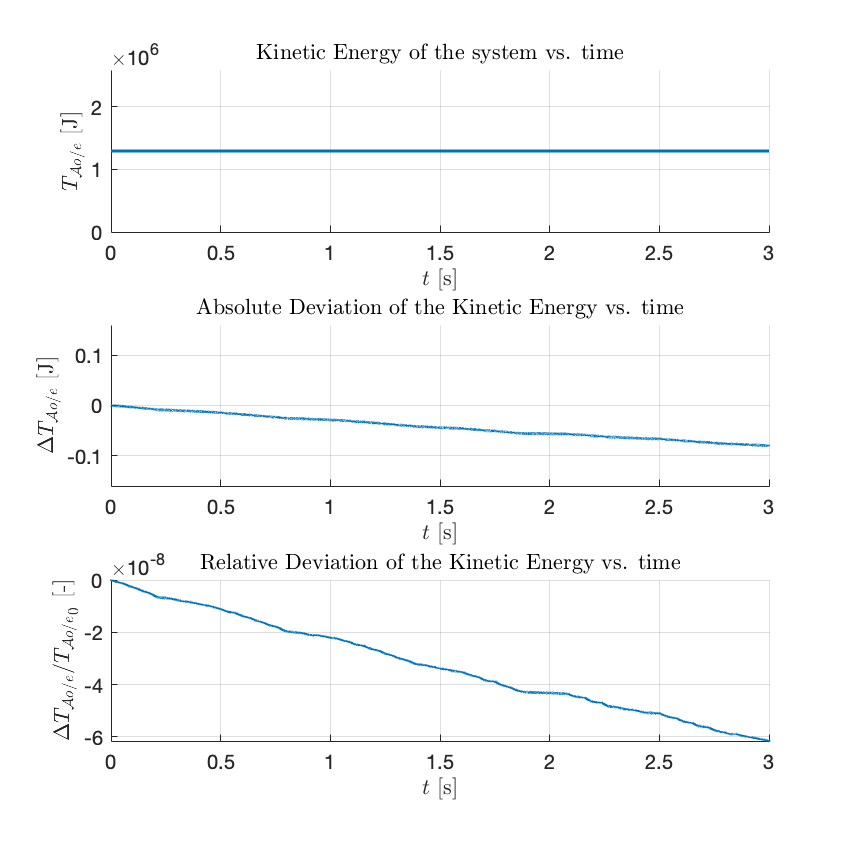
\includegraphics[width=.5\textwidth]{Energy_plot_sys_1e-6.png}
    \caption{Kinetic Energy of the system over time with non-trivial initial conditions and no external forces, integrated with an absolute and relative tolerance of $10^{-6}$.}
    \label{fig:Ekinsyse-6}
\end{figure}
\begin{figure}[p]
    \centering
        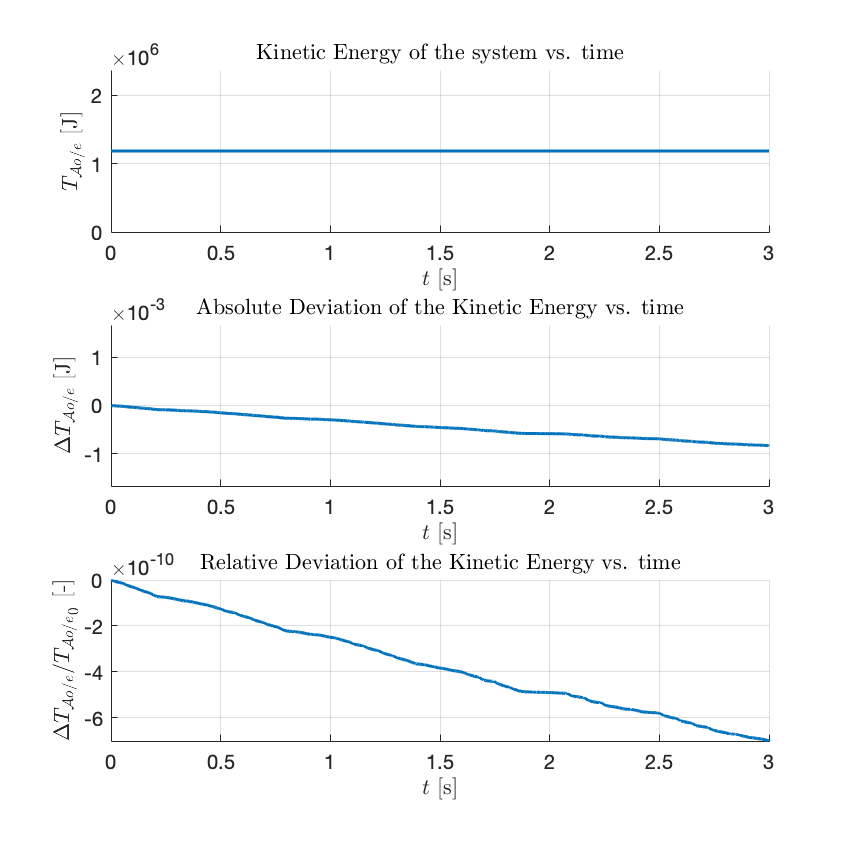
\includegraphics[width=.5\textwidth]{Energy_plot_sys_1e-8.png}
    \caption{Kinetic Energy of the system over time with non-trivial initial conditions and no external forces, integrated with an absolute and relative tolerance of $10^{-8}$.}
    \label{fig:Ekinsyse-8}
\end{figure}
\begin{figure}[!h]
    \centering
        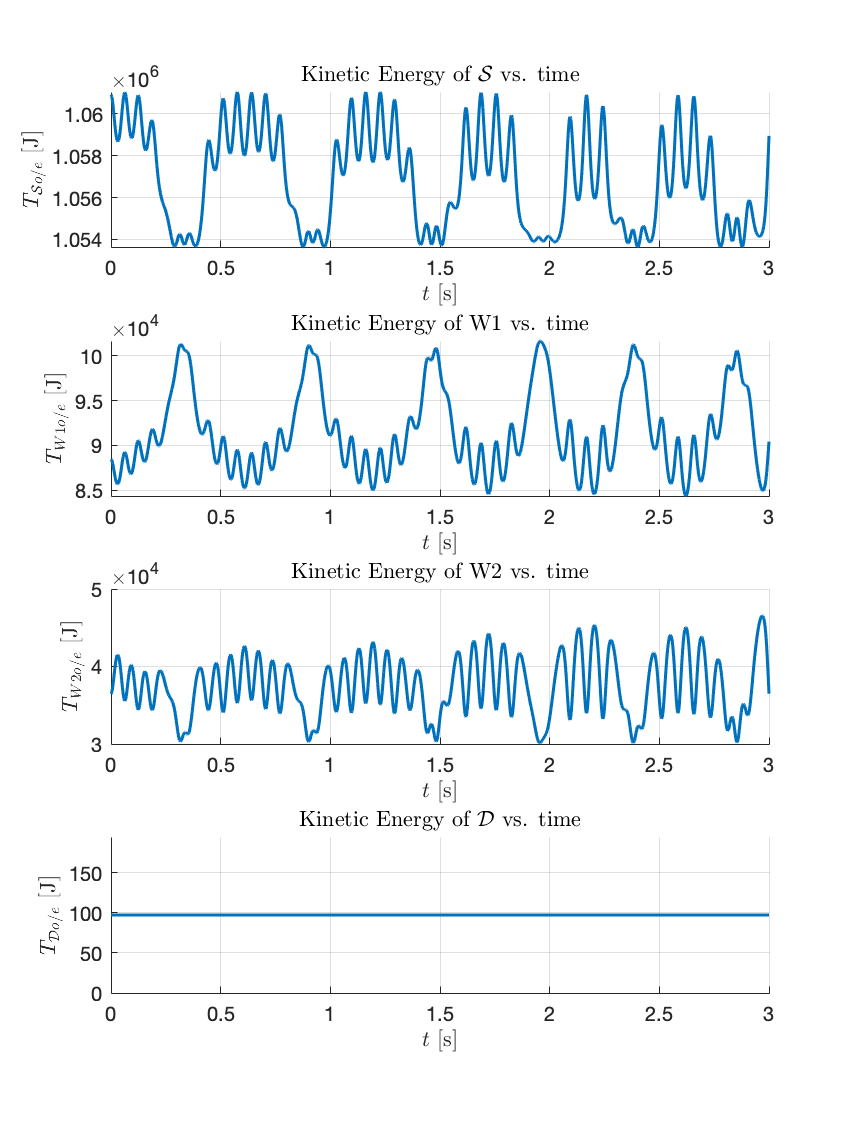
\includegraphics[width=.5\textwidth]{Energy_plot_per_body_1e-8.png}
    \caption{Kinetic Energy of each body over time with non-trivial initial conditions and no external forces, integrated with an absolute and relative tolerance of $10^{-8}$.}
    \label{fig:EkinsysBody}
\end{figure}

%%%%%%%%%%%%%%%%%%%%%%%%%%%%%%%%%%%%%%%%%%%%%%%%%%%%%%%%%%%%%%%%%%%%%%%%%
\section{Conclusion}
The results obtained are in accordance with what one can expect for such a problem. Additional verifications implying non-zero external forces could be made in order to make sure that the forces are correctly implemented. Once this is done, the next step would be to create a controller that drives the state of the system towards the desired state (i.e. the optimal state for the net launch). For this, one could also introduce an observer to take into consideration the inaccuracies introduced by the sensors. A more advanced analysis would also consider the variation of the propellant mass and the gravity acting on the bodies. 
The derivations presented in this report also illustrates the advantages of the Lagrangian approach to Dynamics. In particular, it allows to derive directly the equation of motions in a matrix format, which can be implemented efficiently in \textsc{Matlab}. In addition, the null space method simplifies greatly the problem since the Lagrange multipliers do not have to be implicitly computed.
%%%%%%%%%%%%%%%%%%%%%%%%%%%%%%%%%%%%%%%%%%%%%%%%%%%%%%%%%%%%%%%%%%%%%%%%%
\bibliographystyle{IEEEtran}
\bibliography{refs}
\newpage
\appendix
\small
\begin{align}
\mbf{C}_2(\alpha)&\triangleq\Ctwo{\alpha}  \label{eq:C2}\\ 
\mbf{C}_3(\beta)&\triangleq\Cthree{\beta}   \label{eq:C3} 
\end{align}
\begin{align}
 \mbf{S}_s^{se}&\triangleq\matr
{\mbf{0}}{{\mbf{s}_e^3}^\trans}{\mbf{0}}
{\mbf{0}}{\mbf{0}}{{\mbf{s}_e^1}^\trans}
{{\mbf{s}_e^2}^\trans}{\mbf{0}}{\mbf{0}}
 \label{eq:Ss_se}\\
\mbf{S}_a^{ae}&\triangleq\matr
{\mbf{0}}{{\mbf{a}_e^3}^\trans}{\mbf{0}}
{\mbf{0}}{\mbf{0}}{{\mbf{a}_e^1}^\trans}
{{\mbf{a}_e^2}^\trans}{\mbf{0}}{\mbf{0}}
 \label{eq:Sa_ae}\\
\mbf{S}_b^{be}&\triangleq\matr
{\mbf{0}}{{\mbf{b}_e^3}^\trans}{\mbf{0}}
{\mbf{0}}{\mbf{0}}{{\mbf{b}_e^1}^\trans}
{{\mbf{b}_e^2}^\trans}{\mbf{0}}{\mbf{0}}
 \label{eq:Sb_be}\\
\mbf{S}_d^{de}&\triangleq\matr
{\mbf{0}}{{\mbf{d}_e^3}^\trans}{\mbf{0}}
{\mbf{0}}{\mbf{0}}{{\mbf{d}_e^1}^\trans}
{{\mbf{d}_e^2}^\trans}{\mbf{0}}{\mbf{0}}
 \label{eq:Sd_de}\\
 \mbf{S}_d^{ds}&\triangleq\matr
{\mbf{0}}{{\mbf{d}_s^3}^\trans}{\mbf{0}}
{\mbf{0}}{\mbf{0}}{{\mbf{d}_s^1}^\trans}
{{\mbf{d}_s^2}^\trans}{\mbf{0}}{\mbf{0}}
 \label{eq:Sd_ds}\\
\mbf{S}_a^{as}&\triangleq\mbf{1}_2  \label{eq:Sa_as}\\
\mbf{S}_b^{bs}&\triangleq\mbf{1}_3  \label{eq:Sb_bs}
\end{align}
\begin{align}
\mbs{\Gamma}_s^{se}&\triangleq\matr
{\mbf{0}}{-\mbf{s}_e^3}{\mbf{s}_e^2}
{\mbf{s}_e^3}{\mbf{0}}{-\mbf{s}_e^1}
{-\mbf{s}_e^2}{\mbf{s}_e^1}{\mbf{0}} \label{eq:Gs_se}
\\
\mbs{\Gamma}_a^{ae}&\triangleq\matr
{\mbf{0}}{-\mbf{a}_e^3}{\mbf{a}_e^2}
{\mbf{a}_e^3}{\mbf{0}}{-\mbf{a}_e^1}
{-\mbf{a}_e^2}{\mbf{a}_e^1}{\mbf{0}} \label{eq:Ga_ae}
\\
 \mbs{\Gamma}_b^{be}&\triangleq\matr
{\mbf{0}}{-\mbf{b}_e^3}{\mbf{b}_e^2}
{\mbf{b}_e^3}{\mbf{0}}{-\mbf{b}_e^1}
{-\mbf{b}_e^2}{\mbf{b}_e^1}{\mbf{0}} \label{eq:Gb_be}
\\
\mbs{\Gamma}_d^{de}&\triangleq\matr
{\mbf{0}}{-\mbf{d}_e^3}{\mbf{d}_e^2}
{\mbf{d}_e^3}{\mbf{0}}{-\mbf{d}_e^1}
{-\mbf{d}_e^2}{\mbf{d}_e^1}{\mbf{0}} \label{eq:Gd_de}
\\
\mbs{\Gamma}_d^{ds}&\triangleq\matr
{\mbf{0}}{-\mbf{d}_s^3}{\mbf{d}_s^2}
{\mbf{d}_s^3}{\mbf{0}}{-\mbf{d}_s^1}
{-\mbf{d}_s^2}{\mbf{d}_s^1}{\mbf{0}} \label{eq:Gd_de}
\\
\mbs{\Gamma}_a^{as}&=\mbf{1}_2^\trans \label{eq:Ga_as} \\
\mbs{\Gamma}_b^{bs}&=\mbf{1}_3^\trans \label{eq:Gb_bs}
\end{align}
\beq
\mbs{\Pi}\triangleq \bma{cccccc}
\mbf{1} & \mbf{0} & \mbf{0} & \mbf{0} & \mbf{0} & \mbf{0} \\
\mbf{0} & \mbf{1} & \mbf{0} & \mbf{0} & \mbf{0} & \mbf{0} \\
\mbf{1} & -\mbf{C}_{es}{\mbf{r}_s^{g_1p}}^\times & \mbf{0} & \mbf{0} & \mbf{0} & \mbf{0} \\
\mbf{0} & \mbf{C}_{as} &\mbf{S}_a^{as} & \mbf{0} & \mbf{0} & \mbf{0} \\
\mbf{1} & -\mbf{C}_{es}{\mbf{r}_s^{g_2p}}^\times & \mbf{0} & \mbf{0} & \mbf{0} & \mbf{0} \\
\mbf{0} & \mbf{C}_{bs} & \mbf{0} &\mbf{S}_b^{bs} & \mbf{0} & \mbf{0} \\
\mbf{0} & \mbf{0} & \mbf{0} & \mbf{0} & \mbf{1} & \mbf{0} \\
\mbf{0} & \mbf{0} & \mbf{0} & \mbf{0} & \mbf{0} & \mbf{1}
\ema \label{eq:Pi}
\eeq
\footnotesize
\beq
 \mbs{\Sigma}(\bar{\mbf{q}})\triangleq
\bma{c}
\mbf{r}_e^{po} \\
\mbf{q}^{se} \\
\mbf{r}_e^{po}+\mbf{C}_{es}\mbf{r}_s^{g_1p} \\
\mbf{C}_{es}\mbf{C}_2^\trans(\alpha)\mbf{1}_1 \\
\mbf{C}_{es}\mbf{C}_2^\trans(\alpha)\mbf{1}_2 \\
\mbf{C}_{es}\mbf{C}_2^\trans(\alpha)\mbf{1}_3 \\
\mbf{r}_e^{po}+\mbf{C}_{es}\mbf{r}_s^{g_2p} \\
\mbf{C}_{es}\mbf{C}_3^\trans(\beta)\mbf{1}_1 \\
\mbf{C}_{es}\mbf{C}_3^\trans(\beta)\mbf{1}_2 \\
\mbf{C}_{es}\mbf{C}_3^\trans(\beta)\mbf{1}_3 \\
\mbf{r}_e^{g_do} \\
\mbf{C}_{es}\mbf{C}_{sd}\mbf{1}_1 \\
\mbf{C}_{es}\mbf{C}_{sd}\mbf{1}_2 \\
\mbf{C}_{es}\mbf{C}_{sd}\mbf{1}_3 \\
\mbf{v}_e^{po/e} \\
\mbs{\omega}_s^{se} \\
\dot{\alpha} \\
\dot{\beta} \\
\mbf{v}_e^{g_do} \\
\mbs{\omega}_d^{ds}+\mbf{C}_{sd}^\trans\mbs{\omega}_s^{se}
\ema
\label{eq:Sigma}
\eeq
\begin{align}
\mbs{\digamma}^{\Sp}(\mbf{x})
&\triangleq
\intd_0^{\rho_o} \intd_0^{2\pi} \intd_0^{t_s}\mbf{x} \,\rho_s \dif z_s \dif \theta_s\dif \rho_s 
\nonumber \\ &
\quad+\intd_{(\rho_o-t_s)}^{\rho_o} \intd_0^{2\pi} \intd_{t_s}^{(l_s-t_s)}\mbf{x}\,\rho_s \dif z_s \dif \theta_s\dif \rho_s 
\nonumber \\&
\quad+\intd_0^{\rho_o} \intd_0^{2\pi} \intd_{(l_s-t_s)}^{l_s}\mbf{x} \,\rho_s \dif z_s \dif \theta_s\dif \rho_s
\label{eq:FS}\\
\mbs{\digamma}^{W1}(\mbf{x})
&\triangleq
\intd_0^{\rho_1} \intd_0^{2\pi} \intd_{-\frac{l_1}{2}}^{\frac{l_1}{2}}\mbf{x} \,\rho_a \dif z_a \dif \theta_a\dif \rho_a
\label{eq:FW1}\\
\mbs{\digamma}^{W2}(\mbf{x})
&\triangleq
\intd_0^{\rho_2} \intd_0^{2\pi} \intd_{-\frac{l_2}{2}}^{\frac{l_2}{2}}\mbf{x} \,\rho_b \dif z_b \dif \theta_b\dif \rho_b,
\label{eq:FW2}\\
\mbs{\digamma}^{\De}(\mbf{x})
&\triangleq
\intd_{-\frac{l_d}{2}}^{\frac{l_d}{2}} \intd_{-\frac{l_d}{2}}^{\frac{l_d}{2}} \intd_{-\frac{l_d}{2}}^{\frac{l_d}{2}}\mbf{x} \dif z_d \dif y_d\dif x_d. \label{eq:FD}
\end{align}
\footnotesize
\begin{align}
&\left(\mbf{r}_s^{\dif m_sp^\times}\right)^2=\matr
{-z_s^2-\rho_s^2s^2_{\theta_s}}{\rho_s^2s_{\theta_s}c_{\theta_s}}{z_s\rho_sc_{\theta_s}}
{\rho_s^2s_{\theta_s}c_{\theta_s}}{-z_s^2-\rho_s^2c^2_{\theta_s}}{z_s\rho_ss_{\theta_s}}
{z_s\rho_sc_{\theta_s}}{z_s\rho_ss_{\theta_s}}{-\rho_s^2} \label{eq:rSx}
\\
&\left(\mbf{r}_a^{\dif m_1g_1^\times}\right)^2=\matr
{-z_a^2-\rho_a^2s^2_{\theta_a}}{z_a\rho_ac_{\theta_a}}{\rho_a^2s_{\theta_a}c_{\theta_a}}
{z_a\rho_ac_{\theta_a}}{-\rho_a^2}{z_a\rho_as_{\theta_a}}
{\rho_a^2s_{\theta_a}c_{\theta_a}}{z_a\rho_as_{\theta_a}}{-z_a^2-\rho_a^2c^2_{\theta_a}} \label{eq:rW1x}
\\
&\left(\mbf{r}_b^{\dif m_2g_2^\times}\right)^2=\matr
{-z_b^2-\rho_b^2s^2_{\theta_b}}{\rho_b^2s_{\theta_b}c_{\theta_b}}{z_b\rho_bc_{\theta_b}}
{\rho_b^2s_{\theta_b}c_{\theta_b}}{-z_b^2-\rho_b^2c^2_{\theta_b}}{z_b\rho_bs_{\theta_b}}
{z_b\rho_bc_{\theta_b}}{z_b\rho_bs_{\theta_b}}{-\rho_b^2} \label{eq:rW2x}
\\
&\left(\mbf{r}_d^{\dif m_dg_d^\times}\right)^2=\matr
{-z_d^2-y_d^2}{x_dy_d}{x_dz_d}
{x_dy_d}{-z_d^2-x_d^2}{y_dz_d}
{x_dz_d}{y_dz_d}{-x_d^2-y_d^2} \label{eq:rDx}
\end{align}
\small
\beq
\mbs{\Phi}_{kin}(\mbf{q})
\triangleq \bma{c} 
\mbs{\Phi}_{se}(\mbf{q}^{se}) \\
\mbs{\Phi}_{ae}(\mbf{q}^{ae}) \\
\mbs{\Phi}_{be}(\mbf{q}^{be}) \\
\mbs{\Phi}_{de}(\mbf{q}^{de})
\ema\label{eq:Phikin}
\eeq
\begin{align*}
\mbs{\Phi}_{se}(\mbf{q}^{se})&\triangleq
\bma{c} 
{\mbf{s}_e^1}^\trans\mbf{s}_e^1-1 \\
{\mbf{s}_e^2}^\trans\mbf{s}_e^2-1 \\
{\mbf{s}_e^2}^\trans\mbf{s}_e^1 \\
{\mbf{s}_e^1}^\times\mbf{s}_e^2-\mbf{s}_e^3
\ema &
\mbs{\Phi}_{ae}(\mbf{q}^{ae})&\triangleq
\bma{c} 
{\mbf{a}_e^1}^\trans\mbf{a}_e^1-1 \\
{\mbf{a}_e^2}^\trans\mbf{a}_e^2-1 \\
{\mbf{a}_e^2}^\trans\mbf{a}_e^1 \\
{\mbf{a}_e^1}^\times\mbf{a}_e^2-\mbf{s}_e^3 
\ema \\
\mbs{\Phi}_{be}(\mbf{q}^{be})&\triangleq
\bma{c} 
{\mbf{b}_e^1}^\trans\mbf{b}_e^1-1 \\
{\mbf{b}_e^2}^\trans\mbf{b}_e^2-1 \\
{\mbf{b}_e^2}^\trans\mbf{b}_e^1 \\
{\mbf{b}_e^1}^\times\mbf{b}_e^2-\mbf{s}_e^3
\ema &
\mbs{\Phi}_{de}(\mbf{q}^{de})&\triangleq
\bma{c} 
{\mbf{d}_e^1}^\trans\mbf{d}_e^1-1 \\
{\mbf{d}_e^2}^\trans\mbf{d}_e^2-1 \\
{\mbf{d}_e^2}^\trans\mbf{d}_e^1 \\
{\mbf{d}_e^1}^\times\mbf{d}_e^2-\mbf{d}_s^3
\ema
\end{align*}
\beq
\mbs{\Xi}^{kin}\triangleq\bma{cccccccc}
\mbf{0} & \mbs{\Xi}_s^{se} & \mbf{0} & \mbf{0} & \mbf{0} & \mbf{0} & \mbf{0} & \mbf{0} \\
\mbf{0} & \mbf{0} & \mbf{0} & \mbs{\Xi}_a^{ae} & \mbf{0} & \mbf{0} & \mbf{0} & \mbf{0} \\
\mbf{0} & \mbf{0} & \mbf{0} & \mbf{0} & \mbf{0} & \mbs{\Xi}_b^{be} & \mbf{0} & \mbf{0} \\
\mbf{0} & \mbf{0} & \mbf{0} & \mbf{0} & \mbf{0} & \mbf{0} & \mbf{0} & \mbs{\Xi}_d^{de} 
\ema \label{eq:Xikin}
\eeq
\small
\bdis
\mbs{\Xi}_s^{se} \triangleq
\bma{ccc}
2{\mbf{s}_e^1}^\trans & \mbf{0} & \mbf{0} \\
\mbf{0} & 2{\mbf{s}_e^2}^\trans & \mbf{0} \\
{\mbf{s}_e^2}^\trans & {\mbf{s}_e^1}^\trans & \mbf{0} \\
-{\mbf{s}_e^2}^\times & {\mbf{s}_e^1}^\times & -\mbf{1}
\ema
\quad 
\mbs{\Xi}_a^{ae} \triangleq
\bma{ccc}
2{\mbf{a}_e^1}^\trans & \mbf{0} & \mbf{0} \\
\mbf{0} & 2{\mbf{a}_e^2}^\trans & \mbf{0} \\
{\mbf{a}_e^2}^\trans & {\mbf{a}_e^1}^\trans & \mbf{0} \\
-{\mbf{a}_e^2}^\times & {\mbf{a}_e^1}^\times & -\mbf{1}
\ema
\edis
\bdis
\mbs{\Xi}_b^{be} \triangleq
\bma{ccc}
2{\mbf{b}_e^1}^\trans & \mbf{0} & \mbf{0} \\
\mbf{0} & 2{\mbf{b}_e^2}^\trans & \mbf{0} \\
{\mbf{b}_e^2}^\trans & {\mbf{b}_e^1}^\trans & \mbf{0} \\
-{\mbf{b}_e^2}^\times & {\mbf{b}_e^1}^\times & -\mbf{1}
\ema
\quad
\mbs{\Xi}_d^{de} \triangleq
\bma{ccc}
2{\mbf{d}_e^1}^\trans & \mbf{0} & \mbf{0} \\
\mbf{0} & 2{\mbf{d}_e^2}^\trans & \mbf{0} \\
{\mbf{d}_e^2}^\trans & {\mbf{d}_e^1}^\trans & \mbf{0} \\
-{\mbf{d}_e^2}^\times & {\mbf{d}_e^1}^\times & -\mbf{1}
\ema
\edis
\beq
\mbs{\Xi}^{col}\triangleq\bma{cccccccc}
\mbf{1} & \mbs{\Xi}_{1,2}^{col} & -\mbf{1} & \mbf{0} & \mbf{0} & \mbf{0} & \mbf{0} & \mbf{0} \\
\mbf{1} & \mbs{\Xi}_{2,2}^{col} & \mbf{0} & \mbf{0} & -\mbf{1} & \mbf{0} & \mbf{0} & \mbf{0}
\ema \label{eq:Xicol}
\eeq
\begin{align*}
\mbs{\Xi}_{1,2}^{col}&\triangleq-\mbf{C}_{es}{\mbf{r}_s^{g_1 p}}^\times\mbf{S}_s^{se}, & \mbs{\Xi}_{2,2}^{col}&\triangleq-\mbf{C}_{es}{\mbf{r}_s^{g_2 p}}^\times\mbf{S}_s^{se}.
\end{align*}
\beq
\mbs{\Xi}^{att}\triangleq\bma{cccccccc}
\mbf{0} & \mbs{\Xi}_{1,2}^{att} & \mbf{0} & \mbs{\Xi}_{1,4}^{att} & \mbf{0} & \mbf{0} & \mbf{0} & \mbf{0} \\
\mbf{0} & \mbs{\Xi}_{2,2}^{att} & \mbf{0} & \mbf{0} & \mbf{0} & \mbs{\Xi}_{2,6}^{att}& \mbf{0} & \mbf{0}
\ema \label{eq:Xiatt}
\eeq
\begin{align*}
\mbs{\Xi}_{1,2}^{att}&\triangleq-\colvecc{\mbf{1}_1^\trans}{\mbf{1}_3^\trans}\mbf{C}_{as}\mbf{S}_s^{se},  &\mbs{\Xi}_{1,4}^{att}&\triangleq\colvecc{\mbf{1}_1^\trans}{\mbf{1}_3^\trans}\mbf{S}_a^{ae}, \\
\mbs{\Xi}_{2,2}^{att}&\triangleq-\colvecc{\mbf{1}_1^\trans}{\mbf{1}_2^\trans}\mbf{C}_{bs}\mbf{S}_s^{se}, \quad &\mbs{\Xi}_{2,6}^{att}&\triangleq\colvecc{\mbf{1}_1^\trans}{\mbf{1}_2^\trans}\mbf{S}_b^{be} .
\end{align*}
\beq
\mbf{B}_s\triangleq
\bma{ccccc}
\mbf{s}_e^3 & -\mbf{s}_e^3 & -\mbf{s}_e^3 & \mbf{0} & \mbf{0} \\
\mbf{0} & \mbf{0} & \mbf{0} & \mbf{0} & -\mbf{s}_e^2 \\
\mbf{0} & \rho_s\mbf{s}_e^3 & -\rho_s \mbf{s}_e^3 & \mbf{0} & \mbf{0} \\
\mbf{0} & -l_s\mbf{s}_e^3 & -l_s\mbf{s}_e^3 & -\mbf{s}_e^1 &\mbf{0}
\ema \label{eq:Bs}
\eeq
\beq
\mbf{B}_a\triangleq
\bma{ccccc}
\mbf{0} & \mbf{0} & \mbf{0} & \mbf{0} & \mbf{0} \\
\mbf{0} & \mbf{0} & \mbf{0} & \mbf{0} & \mbf{0} \\
\mbf{0} & \mbf{0} & \mbf{0} & \mbf{0} & \mbf{0} \\
\mbf{0} & \mbf{0} & \mbf{0} & \mbf{a}_e^1 & \mbf{0} 
\ema \label{eq:Ba}
\eeq
\beq
\mbf{B}_b\triangleq
\bma{ccccc}
\mbf{0} & \mbf{0} & \mbf{0} & \mbf{0} & \mbf{0} \\
\mbf{0} & \mbf{0} & \mbf{0} & \mbf{0} & \mbf{b}_e^2 \\
\mbf{0} & \mbf{0} & \mbf{0} & \mbf{0} & \mbf{0} \\
\mbf{0} & \mbf{0} & \mbf{0} & \mbf{0} & \mbf{0} 
\ema \label{eq:Bb}
\eeq
\beq
\dot{\mbf{M}}=\mbox{diag}\{\dot{\mbf{M}}^{\Sp p},\mbf{0},\mbf{0},\mbf{0}\} \label{eq:dM}
\eeq
\bdis
\dot{\mbf{M}}^{\Sp p}=\matrr{\mbf{0}}{-\mbf{C}_{es}{\mbs{\omega}_s^{se}}^\times{\mbf{c}_s^{\Sp p}}^\times}{-{\mbf{c}_s^{\Sp p}}^\times{\mbs{\omega}_s^{se}}^\times\mbf{C}_{es}^\trans}{\mbf{0}}
\edis

\beq
\dot{\mbs{\Pi}}=\bma{cccccc}
\mbf{0} & \mbf{0} & \mbf{0} & \mbf{0} & \mbf{0} & \mbf{0} \\
\mbf{0} & \mbf{0} & \mbf{0} & \mbf{0} & \mbf{0} & \mbf{0} \\
\mbf{0} & \dot{\mbs{\Pi}}_{3,2} & \mbf{0} & \mbf{0} & \mbf{0} & \mbf{0} \\
\mbf{0} & \dot{\mbs{\Pi}}_{4,2} & \mbf{0} & \mbf{0} & \mbf{0} & \mbf{0} \\
\mbf{0} & \dot{\mbs{\Pi}}_{5,2} & \mbf{0} & \mbf{0} & \mbf{0} & \mbf{0} \\
\mbf{0} & \dot{\mbs{\Pi}}_{6,2} & \mbf{0} & \mbf{0} & \mbf{0} & \mbf{0} \\
\mbf{0} & \mbf{0} & \mbf{0} & \mbf{0} & \mbf{0} & \mbf{0} \\
\mbf{0} & \mbf{0} & \mbf{0} & \mbf{0} & \mbf{0} & \mbf{0}
\ema \label{eq:dPi}
\eeq
\footnotesize
\begin{align*}
\dot{\mbs{\Pi}}_{3,2}&=-\mbf{C}_{es}{\mbs{\omega}_s^{se}}^\times{\mbf{r}_s^{g_1p}}^\times \quad & \dot{\mbs{\Pi}}_{4,2}&=-{\mbs{\omega}_a^{as}}^\times\mbf{C}_{as} \\
\dot{\mbs{\Pi}}_{5,2}&=-\mbf{C}_{es}{\mbs{\omega}_s^{se}}^\times{\mbf{r}_s^{g_2p}}^\times \quad & \dot{\mbs{\Pi}}_{6,2}&=-{\mbs{\omega}_b^{bs}}^\times\mbf{C}_{bs}
\end{align*}
\newpage
\begin{table}[t]
\centering
\caption{Initial Conditions} \label{matlab}
\begin{IEEEeqnarraybox}[\IEEEeqnarraystrutmode\IEEEeqnarraystrutsizeadd{2pt}{1pt}]{v/c/v/c/v} \IEEEeqnarrayrulerow\\
&\mbox{Measurable}&&\mbox{Value}&\\
\IEEEeqnarraydblrulerow\\
\IEEEeqnarrayseprow[3pt]\\
& \mbf{r}_e^{po/e}&& \colvec{0}{0}{0} \sii{\meter} &
\IEEEeqnarraystrutsize{0pt}{0pt}\\ \IEEEeqnarrayseprow[3pt]\\
\IEEEeqnarrayrulerow\\
\IEEEeqnarrayseprow[3pt]\\
& \mbf{C}_{es} && \mbf{1}&
\IEEEeqnarraystrutsize{0pt}{0pt}\\ \IEEEeqnarrayseprow[3pt]\\
\IEEEeqnarrayrulerow\\
\IEEEeqnarrayseprow[3pt]\\
& \alpha && 0 \sii{\radian} &
\IEEEeqnarraystrutsize{0pt}{0pt}\\ \IEEEeqnarrayseprow[3pt]\\
\IEEEeqnarrayrulerow\\
\IEEEeqnarrayseprow[3pt]\\
&  \beta && 0 \sii{\radian}&
\IEEEeqnarraystrutsize{0pt}{0pt}\\ \IEEEeqnarrayseprow[3pt]\\
\IEEEeqnarrayrulerow\\
\IEEEeqnarrayseprow[3pt]\\
& \mbf{r}_e^{g_do/e}&& \colvec{0}{0}{0} \sii{\meter} &
\IEEEeqnarraystrutsize{0pt}{0pt}\\ \IEEEeqnarrayseprow[3pt]\\
\IEEEeqnarrayrulerow\\
\IEEEeqnarrayseprow[3pt]\\
& \mbf{C}_{sd} && \mbf{1}&
\IEEEeqnarraystrutsize{0pt}{0pt}\\ \IEEEeqnarrayseprow[3pt]\\
\IEEEeqnarrayrulerow\\
\IEEEeqnarrayseprow[3pt]\\
& \mbf{v}_e^{po/e} && \colvec{10}{0}{0} \sii{\meter\per\sec}&
\IEEEeqnarraystrutsize{0pt}{0pt}\\ \IEEEeqnarrayseprow[3pt]\\
\IEEEeqnarrayrulerow\\
\IEEEeqnarrayseprow[3pt]\\
& \mbs{\omega}_s^{se} && \colvec{0}{\pi}{10\pi} \sii{\radian\per\sec}&
\IEEEeqnarraystrutsize{0pt}{0pt}\\ \IEEEeqnarrayseprow[3pt]\\
\IEEEeqnarrayrulerow\\
\IEEEeqnarrayseprow[3pt]\\
& \dot{\alpha} && 100\pi \sii{\radian\per\sec} &
\IEEEeqnarraystrutsize{0pt}{0pt}\\ \IEEEeqnarrayseprow[3pt]\\
\IEEEeqnarrayrulerow\\
\IEEEeqnarrayseprow[3pt]\\
&  \dot{\beta} && 50\pi \sii{\radian\per\sec}&
\IEEEeqnarraystrutsize{0pt}{0pt}\\ \IEEEeqnarrayseprow[3pt]\\
\IEEEeqnarrayrulerow\\
\IEEEeqnarrayseprow[3pt]\\
& \mbf{v}_e^{g_do/e} && \colvec{10}{0}{0} \sii{\meter\per\sec}&
\IEEEeqnarraystrutsize{0pt}{0pt}\\ \IEEEeqnarrayseprow[3pt]\\
\IEEEeqnarrayrulerow\\
\IEEEeqnarrayseprow[3pt]\\
& \mbs{\omega}_d^{ds} && \colvec{100}{0}{0} \sii{\radian\per\sec}&
\IEEEeqnarraystrutsize{0pt}{0pt}\\
\IEEEeqnarrayseprow[3pt]\\
\IEEEeqnarrayrulerow
\end{IEEEeqnarraybox}
\end{table}

\begin{table}[h]
\centering
\caption{Geometrical Parameters} \label{geom}
\begin{IEEEeqnarraybox}[\IEEEeqnarraystrutmode\IEEEeqnarraystrutsizeadd{2pt}{1pt}]{v/c/v/c/v} \IEEEeqnarrayrulerow\\
&\mbox{Paramter}&&\mbox{Value}&\\
\IEEEeqnarraydblrulerow\\
\IEEEeqnarrayseprow[3pt]\\
& t_s && 0.03 \sii{\meter} &
\IEEEeqnarraystrutsize{0pt}{0pt}\\ \IEEEeqnarrayseprow[3pt]\\
\IEEEeqnarrayrulerow\\
\IEEEeqnarrayseprow[3pt]\\
& \rho_o && 1 \sii{\meter}&
\IEEEeqnarraystrutsize{0pt}{0pt}\\ \IEEEeqnarrayseprow[3pt]\\
\IEEEeqnarrayrulerow\\
\IEEEeqnarrayseprow[3pt]\\
& l_s && 3 \sii{\meter} &
\IEEEeqnarraystrutsize{0pt}{0pt}\\ \IEEEeqnarrayseprow[3pt]\\
\IEEEeqnarrayrulerow\\
\IEEEeqnarrayseprow[3pt]\\
&  \rho_p && 0.5 \sii{\meter}&
\IEEEeqnarraystrutsize{0pt}{0pt}\\ \IEEEeqnarrayseprow[3pt]\\
\IEEEeqnarrayrulerow\\
\IEEEeqnarrayseprow[3pt]\\
& \sigma_s && 2700 \sii{\kilogram\per\cubic\meter} &
\IEEEeqnarraystrutsize{0pt}{0pt}\\ \IEEEeqnarrayseprow[3pt]\\
\IEEEeqnarrayrulerow\\
\IEEEeqnarrayseprow[3pt]\\
& l_1 && 0.1 \sii{\meter}&
\IEEEeqnarraystrutsize{0pt}{0pt}\\ \IEEEeqnarrayseprow[3pt]\\
\IEEEeqnarrayrulerow\\
\IEEEeqnarrayseprow[3pt]\\
& \rho_1 &&0.25 \sii{\meter}&
\IEEEeqnarraystrutsize{0pt}{0pt}\\ \IEEEeqnarrayseprow[3pt]\\
\IEEEeqnarrayrulerow\\
\IEEEeqnarrayseprow[3pt]\\
& z_1 && 1 \sii{\meter}&
\IEEEeqnarraystrutsize{0pt}{0pt}\\ \IEEEeqnarrayseprow[3pt]\\
\IEEEeqnarrayrulerow\\
\IEEEeqnarrayseprow[3pt]\\
& \sigma_1 && 2700 \sii{\kilogram\per\cubic\meter} &
\IEEEeqnarraystrutsize{0pt}{0pt}\\ \IEEEeqnarrayseprow[3pt]\\
\IEEEeqnarrayrulerow\\
\IEEEeqnarrayseprow[3pt]\\
& l_2 && 0.1 \sii{\meter}&
\IEEEeqnarraystrutsize{0pt}{0pt}\\ \IEEEeqnarrayseprow[3pt]\\
\IEEEeqnarrayrulerow\\
\IEEEeqnarrayseprow[3pt]\\
& \rho_2 && 0.25 \sii{\meter} \sii{\meter\per\sec}\hfill&
\IEEEeqnarraystrutsize{0pt}{0pt}\\ \IEEEeqnarrayseprow[3pt]\\
\IEEEeqnarrayrulerow\\
\IEEEeqnarrayseprow[3pt]\\
& z_2 && 2 \sii{\meter}&
\IEEEeqnarraystrutsize{0pt}{0pt}\\ \IEEEeqnarrayseprow[3pt]\\
\IEEEeqnarrayrulerow\\
\IEEEeqnarrayseprow[3pt]\\
& \sigma_2 && 2700 \sii{\kilogram\per\cubic\meter}&
\IEEEeqnarraystrutsize{0pt}{0pt}\\ \IEEEeqnarrayseprow[3pt]\\
\IEEEeqnarrayrulerow\\
\IEEEeqnarrayseprow[3pt]\\
& l_d && 0.2 \sii{\meter}&
\IEEEeqnarraystrutsize{0pt}{0pt}\\ \IEEEeqnarrayseprow[3pt]\\
\IEEEeqnarrayrulerow\\
\IEEEeqnarrayseprow[3pt]\\
& \sigma_d && 2700 \sii{\kilogram\per\cubic\meter} &
\IEEEeqnarraystrutsize{0pt}{0pt}\\
\IEEEeqnarrayseprow[3pt]\\
\IEEEeqnarrayrulerow
\end{IEEEeqnarraybox}
\end{table}
\end{document}


